\documentclass[10pt,a4paper]{article}
\usepackage[UTF8, fontset = none]{ctex}
\setCJKmainfont[BoldFont=黑体,ItalicFont=楷体]{华文中宋}
\usepackage{amssymb,amsmath,amsfonts,amsthm,mathrsfs,dsfont,graphicx}
\usepackage{ifthen,indentfirst,enumerate,color,titletoc}
\usepackage{tikz}
\usepackage{multicol}
\usepackage{makecell}
\usepackage{longtable}
\usepackage{ifthen}
\usetikzlibrary{arrows,calc,intersections,patterns,decorations.pathreplacing,3d,angles,quotes}
\usepackage[bf,small,indentafter,pagestyles]{titlesec}
\usepackage[top=1in, bottom=1in,left=0.8in,right=0.8in]{geometry}
\renewcommand{\baselinestretch}{2}
\newtheorem{defi}{定义~}
\newtheorem{eg}{例~}
\newtheorem{ex}{~}
\newtheorem{rem}{注~}
\newtheorem{thm}{定理~}
\newtheorem{coro}{推论~}
\newtheorem{axiom}{公理~}
\newtheorem{prop}{性质~}
\newcommand{\blank}[1]{\underline{\hbox to #1pt{}}}
\newcommand{\bracket}[1]{(\hbox to #1pt{})}
\newcommand{\onech}[4]{\par\begin{tabular}{p{.9\textwidth}}
A.~#1\\
B.~#2\\
C.~#3\\
D.~#4
\end{tabular}}
\newcommand{\twoch}[4]{\par\begin{tabular}{p{.46\textwidth}p{.46\textwidth}}
A.~#1& B.~#2\\
C.~#3& D.~#4
\end{tabular}}
\newcommand{\vartwoch}[4]{\par\begin{tabular}{p{.46\textwidth}p{.46\textwidth}}
(1)~#1& (2)~#2\\
(3)~#3& (4)~#4
\end{tabular}}
\newcommand{\fourch}[4]{\par\begin{tabular}{p{.23\textwidth}p{.23\textwidth}p{.23\textwidth}p{.23\textwidth}}
A.~#1 &B.~#2& C.~#3& D.~#4
\end{tabular}}
\newcommand{\varfourch}[4]{\par\begin{tabular}{p{.23\textwidth}p{.23\textwidth}p{.23\textwidth}p{.23\textwidth}}
(1)~#1 &(2)~#2& (3)~#3& (4)~#4
\end{tabular}}
\begin{document}

\begin{enumerate}[1.]

\item 如图, 观察长方体$ABCD-A_1B_1C_1D_1$中的点、线、面, 用适当的符号或字母填空:
\begin{center}
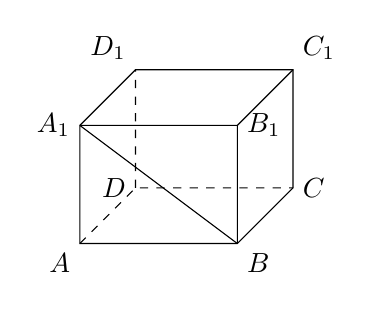
\begin{tikzpicture}[>=latex]
\draw (0,0) node [below left] {$A$} coordinate (A) --++ (2,0) node [below right] {$B$} coordinate (B) --++ (45:{2/2}) node [right] {$C$} coordinate (C)
--++ (0,1.5) node [above right] {$C_1$} coordinate (C1)
--++ (-2,0) node [above left] {$D_1$} coordinate (D1) --++ (225:{2/2}) node [left] {$A_1$} coordinate (A1) -- cycle;
\draw (A) ++ (2,1.5) node [right] {$B_1$} coordinate (B1) -- (B) (B1) --++ (45:{2/2}) (B1) --++ (-2,0);
\draw [dashed] (A) --++ (45:{2/2}) node [left] {$D$} coordinate (D) --++ (2,0) (D) --++ (0,1.5);
\draw (A1) -- (B);
\end{tikzpicture}
\end{center}
(1) 点$B$\blank{20}直线$BC$;\\
(2) 点$A$\blank{20}直线$BC$;\\
(3) 点$D$\blank{20}平面$ABCD$;\\
(4) 点$A_1$\blank{20}平面$ABCD$;\\
(5) 直线$A_1B\cap$直线$BC=$\blank{20};\\
(6) 直线$A_1B\cap$平面$A_1B_1C_1D_1=$\blank{20};\\
(7) 直线$B_1C_1$\blank{20}平面$BB_1C_1C$.
\item 用集合符号表述下列语句, 并将语句所描述的图形画在图中:\\
\begin{center}
\begin{tikzpicture}[>=latex]
\draw (0,0) -- (3,0) --++ (1,1.5) ++ (-0.5,0) node [below] {$\beta$} ++ (0.5,0) --++ (-3,0) -- (0,0);
\draw (0,0) --++ (-1.5,2) --++ (1,1.5) ++ (0.1,-0.2) node [below] {$\alpha$} ++ (-0.1,0.2) --++ (1.5,-2);
\end{tikzpicture}
\end{center}
(1) 点$A$在平面$\alpha$上:\blank{50};\\
(2) 平面$\alpha$经过直线$AC$:\blank{50};\\
(3) 点$B$不在平面$\beta$上:\blank{50};\\
(4) 直线$BC$平行于平面$\beta$:\blank{50}.
\item 下列图形一定是平面图形吗? 请说明理由.\\
(1) 三角形;\\
(2) 梯形;\\
(3) 四边形;\\
(4) 菱形.
\item 判断下列命题的真假:\\
(1) 若空间四点共面, 则其中必有三点共线;\\
(2) 若空间四点中有三点共线, 则此四点必共面;\\
(3) 若空间四点中任何三点不共线, 则此四点不共面;\\
(4) 若空间四点不共面, 则其中任意三点不共线.
\item 证明公理2后的推论2.
\item 平面$\alpha$与平面$\beta$相交于直线$l$, 点$A$、$B$在平面$\alpha$上, 点$C$在平面$\beta$上但不在直线$l$上, 直线$AB$与直线$l$相交于点$R$. 设$A$、$B$、$C$三点确定的平面为$\gamma$, 则$\beta$与$\gamma$的交线是\bracket{20}.
\begin{center}
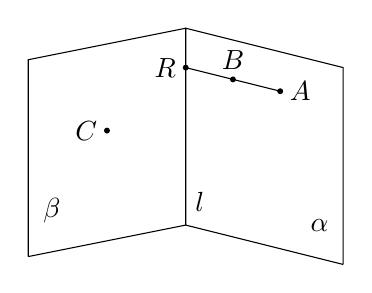
\begin{tikzpicture}[>=latex]
\draw (0,0) -- (2,-0.5) ++ (-0.3,0.3) node [above] {$\alpha$} ++ (0.3,-0.3) --++ (0,2.5) --++ (-2,0.5) -- (0,0) ++ (0,0.3) node [right] {$l$};
\draw (0,0) -- (-2,-0.4) ++ (0.3,0.3) node [above] {$\beta$} ++ (-0.3,-0.3) --++ (0,2.5) --++ (2,0.4);
\filldraw (0,2) circle (0.03) node [left] {$R$} coordinate (R);
\filldraw (1.2,1.7) circle (0.03) node [right] {$A$} coordinate (A);
\filldraw ($(A)!0.5!(R)$) circle (0.03) node [above] {$B$} coordinate (B);
\draw (A) -- (R);
\filldraw (-1,1.2) circle (0.03) node [left] {$C$} coordinate (C);
\end{tikzpicture}
\end{center}
\fourch{直线$AC$}{直线$BC$}{直线$CR$}{以上均不正确}
\item 如图, 已知直线$l$与平面$\alpha$相交于点$O$, $A$、$B \in l$, $C$、$D\in \alpha$, 且$AC\parallel BD$. 求证: $O$、$C$、$D$三点共线.
\begin{center}
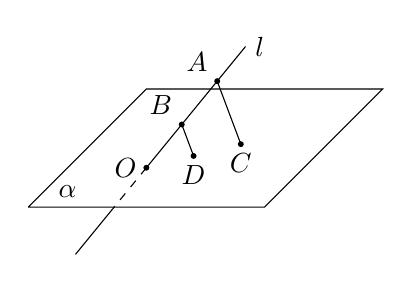
\begin{tikzpicture}[>=latex]
\draw [name path = plane] (0,0) -- (3,0) -- (4.5,1.5) -- (1.5,1.5) -- (0,0) ++ (0.5,0) node [above] {$\alpha$};
\filldraw (1.5,0.5) circle (0.03) node [left] {$O$} coordinate (O);
\filldraw (2.7,0.8) circle (0.03) node [below] {$C$} coordinate (C);
\filldraw ($(O)!0.5!(C)$) circle (0.03) node [below] {$D$} coordinate (D);
\filldraw (2.4,1.6) circle (0.03) node [above left] {$A$} coordinate (A);
\filldraw ($(O)!0.5!(A)$) circle (0.03) node [above left] {$B$} coordinate (B);
\draw (O) -- ($(O)!1.4!(A)$) node [right] {$l$};
\draw (B) -- (D) (A) -- (C);
\path [name path = AO] ($(O)!1.4!(A)$) -- ($(O)!-1!(A)$);
\path [name intersections = {of = AO and plane, by = T}];
\draw [dashed] (O) -- (T);
\draw (T) -- ($(O)!-1!(A)$);
\end{tikzpicture}
\end{center}
\item 画出棱长为$3\text{cm}$的正方体的直观图.
\item $1$个平面把空间分成$2$部分, $2$个平面把空间分成$3$或$4$部分, $3$个平面把空间分成几部分? 
\item 若平面$\alpha$与平面$\beta$、$\gamma$都相交, 则这三个平面的交线可能有几条? 
\fourch{$1$条或$2$条}{$2$条或$3$条}{$1$条或$3$条}{$1$条或$2$条或$3$条}
\item 如图, 在正方体$ABCD-A_1B_1C_1D_1$中, 已知$O$是$DB$的中点, 且直线$A_1C$交平面$C_1BD$于点$M$, 点$C_1$、$M$、$O$的位置关系是\blank{50}.
\begin{center}
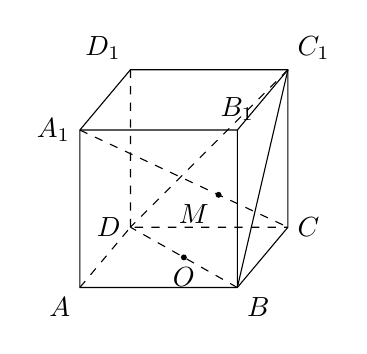
\begin{tikzpicture}[>=latex]
\draw (0,0) node [below left] {$A$} coordinate (A) --++ (2,0) node [below right] {$B$} coordinate (B) --++ (50:{2/2}) node [right] {$C$} coordinate (C)
--++ (0,2) node [above right] {$C_1$} coordinate (C1)
--++ (-2,0) node [above left] {$D_1$} coordinate (D1) --++ (230:{2/2}) node [left] {$A_1$} coordinate (A1) -- cycle;
\draw (A) ++ (2,2) node [above] {$B_1$} coordinate (B1) -- (B) (B1) --++ (50:{2/2}) (B1) --++ (-2,0);
\draw [dashed] (A) --++ (50:{2/2}) node [left] {$D$} coordinate (D) --++ (2,0) (D) --++ (0,2);
\draw (C1) -- (B);
\draw [dashed] (B) -- (D) (C1) -- (D) (A1) -- (C);
\filldraw ($(A1)!{2/3}!(C)$) circle (0.03) node [below left] {$M$} coordinate (M);
\filldraw ($(B)!0.5!(D)$) circle (0.03) node [below] {$O$} coordinate (O);
\end{tikzpicture}
\end{center}
\item 如图, 已知$A\in l$, $B\in l$, $C\in l$, $O\not\in l$. 求证: $OA$、$OB$、$OC$在同一平面上.
\begin{center}
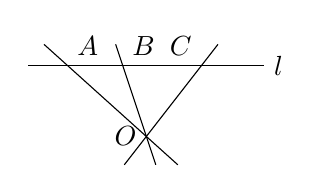
\begin{tikzpicture}[>=latex]
\draw (0,0) -- (3,0) node [right] {$l$};
\draw (0.5,0) node [above right] {$A$} coordinate (A);
\draw (1.2,0) node [above right] {$B$} coordinate (B);
\draw (2.2,0) node [above left] {$C$} coordinate (C);
\draw (1.5,-0.9) node [left] {$O$} coordinate (O);
\draw ($(O)!-0.4!(A)$) -- ($(O)!1.3!(A)$);
\draw ($(O)!-0.4!(B)$) -- ($(O)!1.3!(B)$);
\draw ($(O)!-0.4!(C)$) -- ($(O)!1.3!(C)$);
\end{tikzpicture}
\end{center}
\item 如图, 已知$D$及$E$是$\triangle ABC$的边$AC$及$BC$上的点, 平面$\alpha$经过$D$、$E$两点, 直线$AB$与平面$\alpha$交于点$P$. 求证:点$P$在直线$DE$上.
\begin{center}
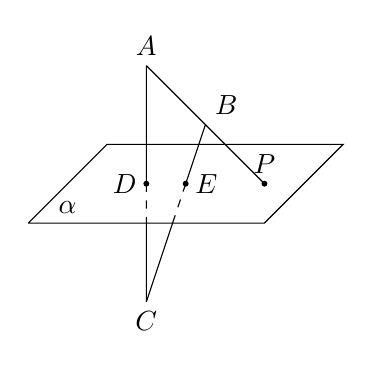
\begin{tikzpicture}[>=latex]
\draw [name path = plane] (0,0) -- (3,0) -- (4,1) -- (1,1) -- (0,0) ++ (0.5,0) node [above] {$\alpha$};
\filldraw (1.5,0.5) circle (0.03) node [left] {$D$} coordinate (D);
\filldraw (3,0.5) circle (0.03) node [above] {$P$} coordinate (P);
\filldraw (2,0.5) circle (0.03) node [right] {$E$} coordinate (E);
\draw (1.5,2) node [above] {$A$} coordinate (A);
\draw ($(A)!0.5!(P)$) node [above right] {$B$} coordinate (B);
\draw (A) -- (P) (B) -- (E) (A) -- (D);
\draw ($(A)!2!(D)$) node [below] {$C$} coordinate (C);
\path [name path = DC] (D) -- (C);
\path [name path = EC] (E) -- (C);
\path [name intersections = {of = DC and plane, by = S}];
\path [name intersections = {of = EC and plane, by = T}];
\draw (S) -- (C) (T) -- (C);
\draw [dashed] (D) -- (S) (E) -- (T);
\end{tikzpicture}
\end{center}
\item 如图, 已知$E$、$F$、$G$、$H$分别是正方体$ABCD-A_1B_1C_1D_1$的棱$AB$、$BC$、$CC_1$、$C_1D_1$的中点, 且$EF$与$HG$相交于点$Q$. 求证:点$Q$在直线$DC$上.
\begin{center}
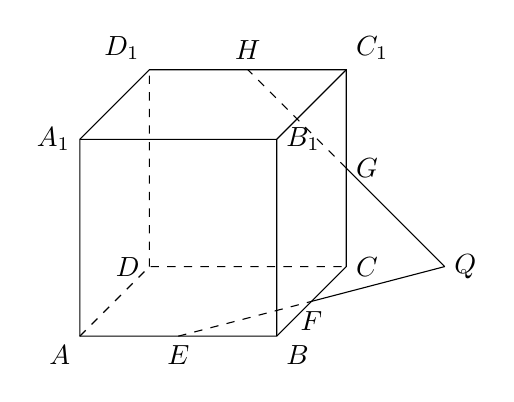
\begin{tikzpicture}[>=latex]
\draw (0,0) node [below left] {$A$} coordinate (A) --++ (2.5,0) node [below right] {$B$} coordinate (B) --++ (45:{2.5/2}) node [right] {$C$} coordinate (C)
--++ (0,2.5) node [above right] {$C_1$} coordinate (C1)
--++ (-2.5,0) node [above left] {$D_1$} coordinate (D1) --++ (225:{2.5/2}) node [left] {$A_1$} coordinate (A1) -- cycle;
\draw (A) ++ (2.5,2.5) node [right] {$B_1$} coordinate (B1) -- (B) (B1) --++ (45:{2.5/2}) (B1) --++ (-2.5,0);
\draw [dashed] (A) --++ (45:{2.5/2}) node [left] {$D$} coordinate (D) --++ (2.5,0) (D) --++ (0,2.5);
\draw ($(D)!1.5!(C)$) node [right] {$Q$} coordinate (Q);
\draw ($(A)!0.5!(B)$) node [below] {$E$} coordinate (E);
\draw ($(C)!0.5!(B)$) node [below] {$F$} coordinate (F);
\draw ($(C)!0.5!(C1)$) node [right] {$G$} coordinate (G);
\draw ($(C1)!0.5!(D1)$) node [above] {$H$} coordinate (H);
\draw [dashed] (E) -- (F) (G) -- (H);
\draw (F) -- (Q) (Q) -- (G);
\end{tikzpicture}
\end{center}
\item 证明公理$2$后的推论$3$.
\item 空间两条互相平行的直线指的是\bracket{20}.
\twoch{在空间没有公共点的两条直线}{分别在两个平面上的两条直线}{在两个不同的平面上且没有公共点的两条直线}{在同一平面上且没有公共点的两条直线}
\item 如图, 在正方体$ABCD-A_1B_1C_1D_1$中, $M$、$N$分别为$CD$、$AD$的中点. 求证: $MN\parallel A_1C_1$.
\begin{center}
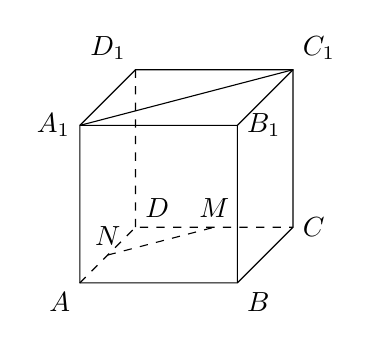
\begin{tikzpicture}[>=latex]
\draw (0,0) node [below left] {$A$} coordinate (A) --++ (2,0) node [below right] {$B$} coordinate (B) --++ (45:{2/2}) node [right] {$C$} coordinate (C)
--++ (0,2) node [above right] {$C_1$} coordinate (C1)
--++ (-2,0) node [above left] {$D_1$} coordinate (D1) --++ (225:{2/2}) node [left] {$A_1$} coordinate (A1) -- cycle;
\draw (A) ++ (2,2) node [right] {$B_1$} coordinate (B1) -- (B) (B1) --++ (45:{2/2}) (B1) --++ (-2,0);
\draw [dashed] (A) --++ (45:{2/2}) node [above right] {$D$} coordinate (D) --++ (2,0) (D) --++ (0,2);
\draw ($(A)!0.5!(D)$) node [above] {$N$} coordinate (N);
\draw ($(C)!0.5!(D)$) node [above] {$M$} coordinate (M);
\draw (A1) -- (C1);
\draw [dashed] (N) -- (M);
\end{tikzpicture}
\end{center}
\item 如图是一个正方体的平面展开图, 在这个正方体中, 下列说法中正确的序号是\blank{50}.
\begin{center}
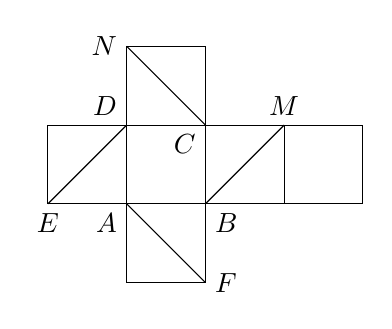
\begin{tikzpicture}[>=latex]
\draw (0,0) node [below] {$E$} rectangle (4,1);
\draw (1,2) node [left] {$N$} rectangle (2,-1) node [right] {$F$};
\draw (3,0) -- (3,1) node [above] {$M$};
\draw (2,0) node [below right] {$B$} -- (3,1);
\draw (1,0) node [below left] {$A$} -- (2,-1);
\draw (0,0) -- (1,1) node [above left] {$D$};
\draw (1,2) -- (2,1) node [below left] {$C$};
\end{tikzpicture}
\end{center}
\textcircled{1} 直线$AF$与直线$DE$相交; \textcircled{2} 直线$CN$与直线$DE$平行; \textcircled{3} 直线$BM$与直线$DE$是异面直线; \textcircled{4}直线$CN$与直线$BM$成$60^\circ$角.
\item 如图, 在正方体$ABCD-A_1B_1C_1D_1$中, $M$、$N$分别是棱$C_1D_1$、$C_1C$的中点. 判断下列结论是否成立, 并说明理由:
\begin{center}
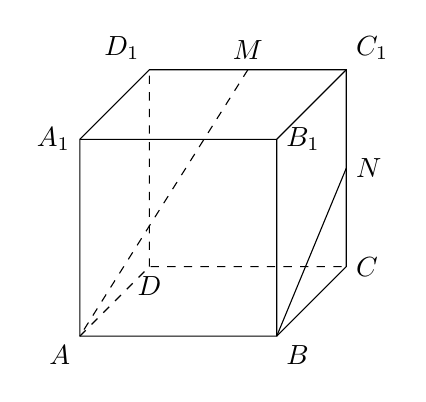
\begin{tikzpicture}[>=latex]
\draw (0,0) node [below left] {$A$} coordinate (A) --++ (2.5,0) node [below right] {$B$} coordinate (B) --++ (45:{2.5/2}) node [right] {$C$} coordinate (C)
--++ (0,2.5) node [above right] {$C_1$} coordinate (C1)
--++ (-2.5,0) node [above left] {$D_1$} coordinate (D1) --++ (225:{2.5/2}) node [left] {$A_1$} coordinate (A1) -- cycle;
\draw (A) ++ (2.5,2.5) node [right] {$B_1$} coordinate (B1) -- (B) (B1) --++ (45:{2.5/2}) (B1) --++ (-2.5,0);
\draw [dashed] (A) --++ (45:{2.5/2}) node [below] {$D$} coordinate (D) --++ (2.5,0) (D) --++ (0,2.5);
\draw ($(C)!0.5!(C1)$) node [right] {$N$} coordinate (N) -- (B);
\draw [dashed] ($(C1)!0.5!(D1)$) node [above] {$M$} coordinate (M) -- (A);
\end{tikzpicture}
\end{center}
(1) 直线$AM$与$CC_1$是相交直线;\\
(2) 直线$AM$与$BN$是平行直线;\\
(3) 直线$AM$与$DD_1$是异面直线.
\item 已知$A$、$B$、$C$、$D$是空间四个点, 且直线$AB$与$CD$是两条异面直线. 求证: 直线$AC$与$BD$也是异面直线.
\item 如图, 在四面体$ABCD$中, $AB=CD$, $AB\perp CD$, $E$、$F$分别为$BC$、$AD$的中点. 求直线$EF$和$AB$所成角的大小.
\begin{center}
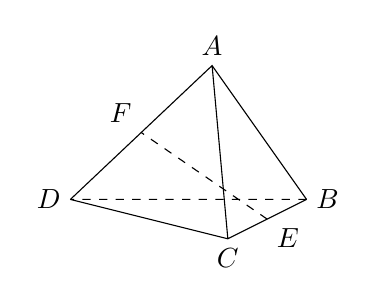
\begin{tikzpicture}[>=latex]
\draw (0,0) node [left] {$D$} coordinate (D);
\draw (3,0) node [right] {$B$} coordinate (B);
\draw (1.8,1.7) node [above] {$A$} coordinate (A);
\draw (2,-0.5) node [below] {$C$} coordinate (C);
\draw ($(B)!0.5!(C)$) node [below right] {$E$} coordinate (E);
\draw ($(A)!0.5!(D)$) node [above left] {$F$} coordinate (F);
\draw (A) -- (C) (B) -- (C) -- (D) (D) -- (A) -- (B);
\draw [dashed] (E) -- (F) (B) -- (D);
\end{tikzpicture}
\end{center}
\item 如果两个三角形不在同一平面上, 它们的边两两对应平行, 那么这两个三角形\bracket{20}.
\fourch{全等}{相似}{相似但不全等}{不相似}
\item 如图, 在正方体$ABCD-A_1B_1C_1D_1$中, $E$、$F$、$G$分别是$AB$、$BB_1$、$BC$的中点.求证: $\triangle EFG\sim\triangle C_1DA_1$.
\begin{center}
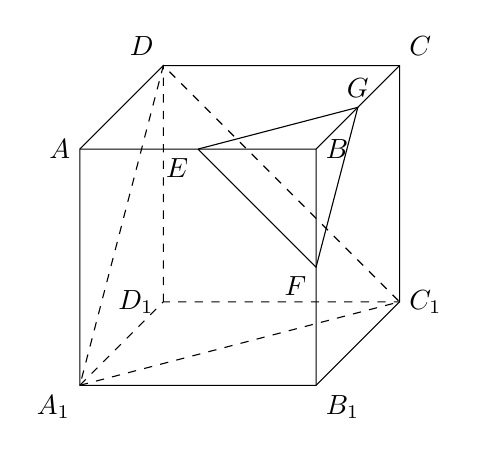
\begin{tikzpicture}[>=latex]
\draw (0,0) node [below left] {$A_1$} coordinate (A) --++ (3,0) node [below right] {$B_1$} coordinate (B) --++ (45:{3/2}) node [right] {$C_1$} coordinate (C)
--++ (0,3) node [above right] {$C$} coordinate (C1)
--++ (-3,0) node [above left] {$D$} coordinate (D1) --++ (225:{3/2}) node [left] {$A$} coordinate (A1) -- cycle;
\draw (A) ++ (3,3) node [right] {$B$} coordinate (B1) -- (B) (B1) --++ (45:{3/2}) (B1) --++ (-3,0);
\draw [dashed] (A) --++ (45:{3/2}) node [left] {$D_1$} coordinate (D) --++ (3,0) (D) --++ (0,3);
\draw [dashed] (A) -- (C) -- (D1) -- (A);
\draw ($(A1)!0.5!(B1)$) node [below left] {$E$} coordinate (E);
\draw ($(B1)!0.5!(B)$) node [below left] {$F$} coordinate (F);
\draw ($(B1)!0.5!(C1)$) node [above] {$G$} coordinate (G);
\draw (E) -- (F) -- (G) -- (E);
\end{tikzpicture}
\end{center}
\item 如图, 在长方体$ABCD-A_1B_1C_1D_1$中, 判断下列直线的位置关系:
\begin{center}
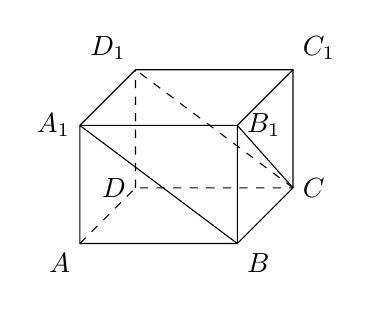
\begin{tikzpicture}[>=latex]
\draw (0,0) node [below left] {$A$} coordinate (A) --++ (2,0) node [below right] {$B$} coordinate (B) --++ (45:{2/2}) node [right] {$C$} coordinate (C)
--++ (0,1.5) node [above right] {$C_1$} coordinate (C1)
--++ (-2,0) node [above left] {$D_1$} coordinate (D1) --++ (225:{2/2}) node [left] {$A_1$} coordinate (A1) -- cycle;
\draw (A) ++ (2,1.5) node [right] {$B_1$} coordinate (B1) -- (B) (B1) --++ (45:{2/2}) (B1) --++ (-2,0);
\draw [dashed] (A) --++ (45:{2/2}) node [left] {$D$} coordinate (D) --++ (2,0) (D) --++ (0,1.5);
\draw (A1) -- (B) (B1) -- (C);
\draw [dashed] (C) -- (D1);
\end{tikzpicture}
\end{center}
(1) 直线$A_1B$与直线$D_1C$的位置关系是\blank{50};\\
(2) 直线$A_1B$与直线$B_1C$的位置关系是\blank{50};\\
(3) 直线$D_1D$与直线$D_1C$的位置关系是\blank{50};\\
(4) 直线$AB$与直线$B_1C$的位置关系是\blank{50}.
\item 如图, 已知不在同一平面上的三条直线$a$、$b$、$c$相交于点$O$, $M$、$P$是直线$a$上的两点, $N$、$Q$分别是直线$b$、$c$上与点$O$不重合的点. 求证: $MN$和$PQ$是异面直线.
\begin{center}
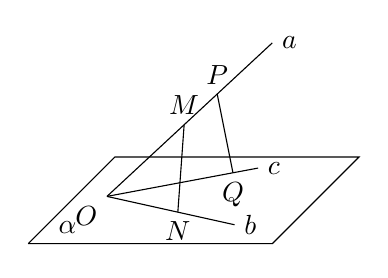
\begin{tikzpicture}[>=latex]
\draw (0.3,0.6) --++ (3.1,0) --++ (1.1,1.1) --++ (-3.1,0) -- (0.3,0.6) ++ (0.5,0) node [above] {$\alpha$};
\draw (1.3,1.2) node [below left] {$O$} coordinate (O);
\draw (2.7,2.5) node [above] {$P$} coordinate (P);
\draw ($(O)!0.7!(P)$) node [above] {$M$} coordinate (M);
\draw (O) -- ($(O)!1.5!(P)$) node [right] {$a$} coordinate (a);
\draw (2.2,1) node [below] {$N$} coordinate (N);
\draw (2.9,1.5) node [below] {$Q$} coordinate (Q);
\draw (O) -- ($(O)!1.8!(N)$) node [right] {$b$} coordinate (b);
\draw (O) -- ($(O)!1.2!(Q)$) node [right] {$c$} coordinate (c);
\draw (M) -- (N) (P) -- (Q);
\end{tikzpicture}
\end{center}
\item 如图, 在四面体$ABCD$中, $AC=8$, $BD=6$, $M$、$N$分别为$AB$、$CD$的中点, 并且异面直线$AC$与$BD$所成的角为$90^\circ$. 求$MN$的长.
\begin{center}
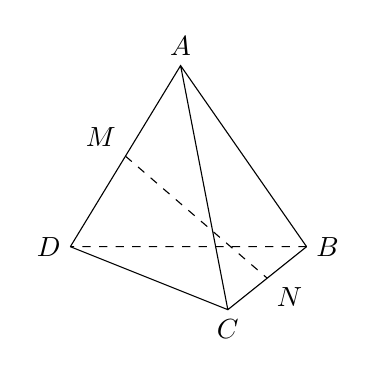
\begin{tikzpicture}[>=latex]
\draw (0,0) node [left] {$D$} coordinate (D);
\draw (3,0) node [right] {$B$} coordinate (B);
\draw (1.4,2.3) node [above] {$A$} coordinate (A);
\draw (2,-0.8) node [below] {$C$} coordinate (C);
\draw ($(B)!0.5!(C)$) node [below right] {$N$} coordinate (N);
\draw ($(A)!0.5!(D)$) node [above left] {$M$} coordinate (M);
\draw (A) -- (C) (B) -- (C) -- (D) (D) -- (A) -- (B);
\draw [dashed] (M) -- (N) (B) -- (D);
\end{tikzpicture}
\end{center}
\item 如图, 在空间四边形$ABCD$中, $E$、$F$、$G$、$H$分别是边$AB$、$BC$、$CD$、$DA$的中点. 当对角线$AC$和$BD$满足什么条件时, $EFGH$分别是矩形、菱形、正方形?
\begin{center}
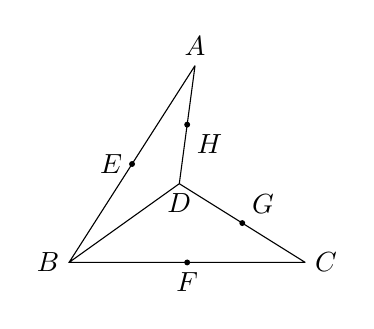
\begin{tikzpicture}[>=latex]
\draw (0,0) node [left] {$B$} coordinate (B);
\draw (3,0) node [right] {$C$} coordinate (C);
\draw (1.4,1) node [below] {$D$} coordinate (D);
\draw (1.6,2.5) node [above] {$A$} coordinate (A);
\filldraw ($(A)!0.5!(B)$) circle (0.03) node [left] {$E$} coordinate (E);
\filldraw ($(B)!0.5!(C)$) circle (0.03) node [below] {$F$} coordinate (F);
\filldraw ($(C)!0.5!(D)$) circle (0.03) node [above right] {$G$} coordinate (G);
\filldraw ($(D)!0.5!(A)$) circle (0.03) node [below right] {$H$} coordinate (H);
\draw (A) -- (B) -- (C) (A) -- (D) -- (C) (B) -- (D);
\end{tikzpicture}
\end{center}
\item 如图, 在长方体$ABCD-A_1B_1C_1D_1$中, $E$是棱$DD_1$的中点, 试判断$BD_1$与平面$AEC$的位置关系, 并说明理由.
\begin{center}
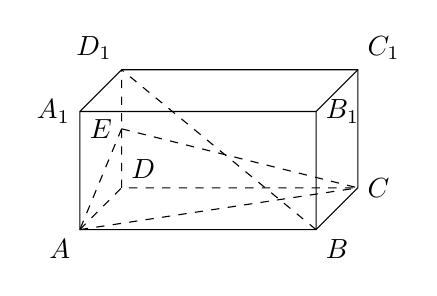
\begin{tikzpicture}[>=latex]
\draw (0,0) node [below left] {$A$} coordinate (A) --++ (3,0) node [below right] {$B$} coordinate (B) --++ (45:{1.5/2}) node [right] {$C$} coordinate (C)
--++ (0,1.5) node [above right] {$C_1$} coordinate (C1)
--++ (-3,0) node [above left] {$D_1$} coordinate (D1) --++ (225:{1.5/2}) node [left] {$A_1$} coordinate (A1) -- cycle;
\draw (A) ++ (3,1.5) node [right] {$B_1$} coordinate (B1) -- (B) (B1) --++ (45:{1.5/2}) (B1) --++ (-3,0);
\draw [dashed] (A) --++ (45:{1.5/2}) node [above right] {$D$} coordinate (D) --++ (3,0) (D) --++ (0,1.5);
\draw [dashed] (B) -- (D1);
\draw ($(D)!0.5!(D1)$) node [left] {$E$} coordinate (E);
\draw [dashed] (E) -- (A) (E) -- (C) (A) -- (C);
\end{tikzpicture}
\end{center}
\item 在长方体$ABCD-A_1B_1C_1D_1$中, $M$、$N$分别为矩形$A_1ADD_1$和$D_1C_1CD$的中心. 求证: $MN\parallel$平面$ABCD$.
\item 如图, $\alpha\cap \beta=CD$, $\alpha\cap \gamma=EF$, $\beta\cap \gamma=AB$, $AB\parallel \alpha$. 求证: $CD\parallel EF$.
\begin{center}
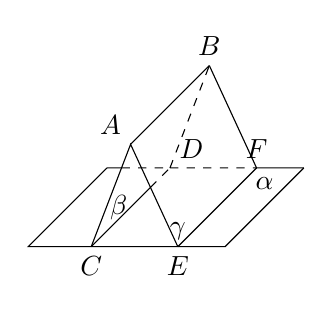
\begin{tikzpicture}[>=latex]
\path [name path = plane]  (1,1) --++ (2.5,0);
\draw (1,1) -- (0,0) -- (2.5,0) --++ (1,1);
\draw (0.8,0) node [below] {$C$} coordinate (C);
\draw (1.9,0) node [below] {$E$} coordinate (E);
\draw (1.3,1.3) node [above left] {$A$} coordinate (A);
\draw (C) -- (A) -- (E);
\draw (A) --++ (1,1) node [above] {$B$} coordinate (B);
\draw (E) --++ (1,1) node [above] {$F$} coordinate (F);
\path [name path = CD] (C) --++ (1,1) node [above right] {$D$}coordinate (D);
\path [name path = CA] (C) -- (A);
\path [name path = EA] (E) -- (A);
\draw (B) -- (F) -- (3.5,1);
\draw [dashed] (D) -- (B) (D) -- (F);
\path [name intersections = {of = CA and plane, by = S}];
\path [name intersections = {of = CD and EA, by = T}];
\draw (S) -- (1,1) (C) -- (T);
\draw [dashed] (S) -- (D) (T) -- (D);
\draw (C) ++ (0.35,0.5) node {$\beta$};
\draw (E) ++ (0,0.2) node {$\gamma$};
\draw (3,1) node [below] {$\alpha$};
\end{tikzpicture}
\end{center}
\item 已知$E$、$F$分别是空间四边形$ABCD$的边$BC$、$AD$的中点, 过直线$EF$且平行于$AB$的平面与$AC$交于点$G$. 求证: $G$是$AC$的中点.
\item 证明:如果直线$l\parallel$平面$\alpha$, 那么$l$上任意两点到平面$\alpha$的距离都相等.
\item 已知平面$\alpha$与平面$\beta$相交于直线$AB$, 直线$PC$垂直于平面$\alpha$, 直线$PD$垂直于平面$\beta$, 其垂足分别为$C$、$D$. 求证: $AB\perp CD$.
\item 由平面$\alpha$外一点$A$向$\alpha$分别引斜线段$AB$、$AC$, 已知这两条斜线段和平面$\alpha$所成角的大小之比为$2: 1$, 而它们的长度之比为$2: 3$. 分别求斜线段$AB$、$AC$和平面$\alpha$所成角的大小.
\item 从平面外一点$D$向该平面引垂线段$DA$及斜线段$DB$、$DC$, 已知$DA$的长为$a$, $\angle BDA=\angle CDA=60^\circ$, $\angle BDC=90^\circ$. 求$BC$的长.
\item 证明: 两条平行直线和同一个平面所成的角相等.
\item 在正方体$ABCD-A_1B_1C_1D_1$中, 求证: $D_1B\perp$平面$AB_1C$.
\item 如图, 在四面体$ABCD$中, $E$、$F$分别是$\triangle ACD$、$\triangle BCD$的重心. 该四面体中, 哪些面与$EF$平行? 请说明理由.
\begin{center}
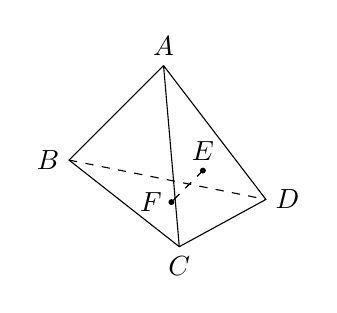
\begin{tikzpicture}[>=latex]
\draw (0,0) node [left] {$B$} coordinate (B);
\draw (2.5,-0.5) node [right] {$D$} coordinate (D);
\draw (1.2,1.2) node [above] {$A$} coordinate (A);
\draw (1.4,-1.1) node [below] {$C$} coordinate (C);
\filldraw ($(B)!{2/3}!($(C)!0.5!(D)$)$) circle (0.03) node [left]  {$F$} coordinate (F);
\filldraw ($(C)!{2/3}!($(A)!0.5!(D)$)$) circle (0.03) node [above]  {$E$} coordinate (E);
\draw (A) -- (B) -- (C) -- (D) -- (A) (A) -- (C);
\draw [dashed] (B) -- (D) (E) -- (F);
\end{tikzpicture}
\end{center}
\item 如图, 已知$BD$是$\odot O$的直径, 点$C$是$\odot O$上的动点. 设过动点$C$的直线$AC$垂直于$\odot O$所在的平面, 且$E$、$F$分别是边$AC$、$AD$的中点. 求证: $EF\perp$平面$ABC$.
\begin{center}
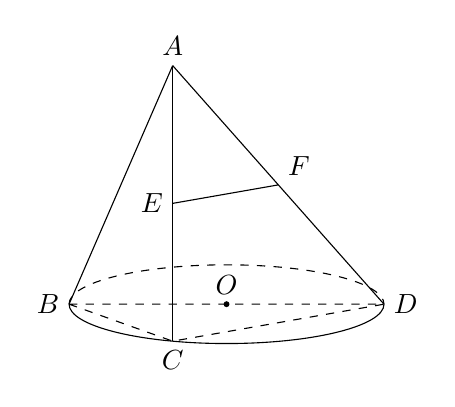
\begin{tikzpicture}[>=latex]
\filldraw (0,0) circle (0.03) node [above] {$O$} coordinate (O);
\draw (-2,0) node [left] {$B$} coordinate (B) arc (180:360:2 and 0.5) node [right] {$D$} coordinate (D);
\draw [dashed] (-2,0) arc (180:0:2 and 0.5);
\draw ({2*cos(250)},{0.5*sin(250)}) node [below] {$C$} coordinate (C) --++ (0,3.5) node [above] {$A$} coordinate (A);
\draw ($(A)!0.5!(C)$) node [left] {$E$} coordinate (E);
\draw ($(A)!0.5!(D)$) node [above right] {$F$} coordinate (F);
\draw (A) -- (B) (A) -- (D) (E) -- (F);
\draw [dashed] (B) -- (D) (B) -- (C) -- (D);
\end{tikzpicture}
\end{center}
\item 如图, 在棱长为$1$的正方体$ABCD-A_1B_1C_1D_1$中, $E$、$F$及$G$分别为棱$BB_1$、$DD_1$和$CC_1$的中点.
\begin{center}
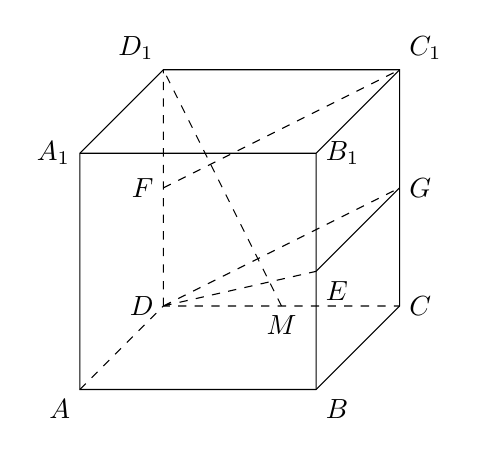
\begin{tikzpicture}[>=latex]
\draw (0,0) node [below left] {$A$} coordinate (A) --++ (3,0) node [below right] {$B$} coordinate (B) --++ (45:{3/2}) node [right] {$C$} coordinate (C)
--++ (0,3) node [above right] {$C_1$} coordinate (C1)
--++ (-3,0) node [above left] {$D_1$} coordinate (D1) --++ (225:{3/2}) node [left] {$A_1$} coordinate (A1) -- cycle;
\draw (A) ++ (3,3) node [right] {$B_1$} coordinate (B1) -- (B) (B1) --++ (45:{3/2}) (B1) --++ (-3,0);
\draw [dashed] (A) --++ (45:{3/2}) node [left] {$D$} coordinate (D) --++ (3,0) (D) --++ (0,3);
\draw ($(B)!0.5!(B1)$)node [below right] {$E$} coordinate (E) -- ($(C)!0.5!(C1)$) node [right] {$G$} coordinate (G);
\draw [dashed] (D) -- (E) (D) -- (G);
\draw [dashed] ($(D)!0.5!(D1)$) node [left] {$F$} coordinate (F) -- (C1);
\draw [dashed] ($(C)!0.5!(D)$) node [below] {$M$} coordinate (M) -- (D1);
\end{tikzpicture}
\end{center}
(1) 求证: $C_1F\parallel$平面$DEG$;\\
(2) 试在棱$CD$上取一点$M$, 使$D_1M\perp$平面$DEG$.
\item 经过一个角的顶点引这个角所在平面的斜线. 如果此斜线和这个角两边的夹角相等, 求证: 该斜线在平面上的投影是这个角的角平分线所在的直线.
\item 如图, 在$\triangle ABC$中, $\angle ACB=90^\circ$, 且$DA$垂直于$\triangle ABC$所在的平面$\alpha$, $M$、$N$分别是边$AC$、$DB$的中点.求证: $MN\perp AC$.
\begin{center}
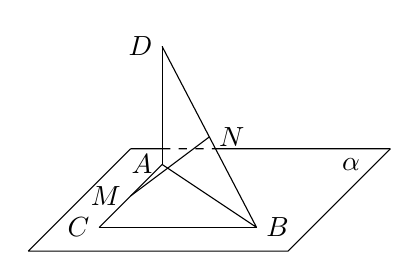
\begin{tikzpicture}[>=latex]
\draw (0,0) node [left] {$C$} coordinate (C) -- (2,0) node [right] {$B$} coordinate (B);
\draw (0.8,0.8) node [left] {$A$} coordinate (A) --++ (0,1.5) node [left] {$D$} coordinate (D);
\draw (A) -- (C) (A) -- (B) (B) -- (D);
\draw ($(A)!0.5!(C)$) node [left] {$M$} coordinate (M);
\draw ($(B)!0.5!(D)$) node [right] {$N$} coordinate (N);
\draw (M) -- (N);
\draw (-0.9,-0.3) --++ (3.3,0) --++ (1.3,1.3) coordinate (R) ++ (-3.3,0) coordinate (P) --++ (-1.3,-1.3);
\path [name path = rear] (R) --++ (-3.3,0);
\path [name path = BD] (B) -- (D);
\path [name path = AD] (A) -- (D);
\path [name intersections = {of = AD and rear, by = S}];
\path [name intersections = {of = BD and rear, by = T}];
\draw (S) -- (P) (T) -- (R);
\draw [dashed] (S) -- (T);
\draw (R) ++ (-0.5,0) node [below] {$\alpha$};
\end{tikzpicture}
\end{center}
\item 判断下列命题的真假, 并说明理由:\\
(1) 平行于同一条直线的两个平面平行;\\
(2) 若两个平面分别经过两条平行直线, 则这两个平面平行;\\
(3) 分别在两个平行平面上的两条直线平行;\\
(4) 与两条异面直线都平行的两个平面平行.
\item 如图, 在正方体$ABCD-A_1B_1C_1D_1$中, $AE=A_1E_1$, $AF=A_1F_1$. 求证: $ EF\parallel E_1F_1$, 且$EF=E_1F_1$.
\begin{center}
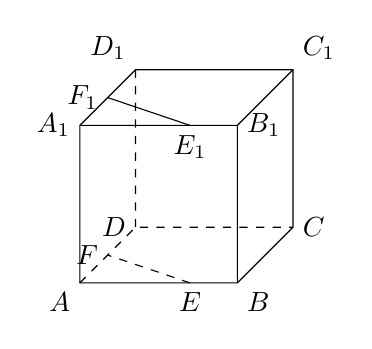
\begin{tikzpicture}[>=latex]
\draw (0,0) node [below left] {$A$} coordinate (A) --++ (2,0) node [below right] {$B$} coordinate (B) --++ (45:{2/2}) node [right] {$C$} coordinate (C)
--++ (0,2) node [above right] {$C_1$} coordinate (C1)
--++ (-2,0) node [above left] {$D_1$} coordinate (D1) --++ (225:{2/2}) node [left] {$A_1$} coordinate (A1) -- cycle;
\draw (A) ++ (2,2) node [right] {$B_1$} coordinate (B1) -- (B) (B1) --++ (45:{2/2}) (B1) --++ (-2,0);
\draw [dashed] (A) --++ (45:{2/2}) node [left] {$D$} coordinate (D) --++ (2,0) (D) --++ (0,2);
\draw ($(A)!0.7!(B)$) node [below] {$E$} coordinate (E);
\draw ($(A1)!0.7!(B1)$) node [below] {$E_1$} coordinate (E1);
\draw ($(A)!0.5!(D)$) node [left] {$F$} coordinate (F);
\draw ($(A1)!0.5!(D1)$) node [left] {$F_1$} coordinate (F1);
\draw (E1) -- (F1);
\draw [dashed] (E) -- (F);
\end{tikzpicture}
\end{center}
\item 如图, $A$、$B$、$C$为不共线的三点, $AA_1\parallel BB_1\parallel CC_1$, 且$AA_1=BB_1=CC_1$. 求证: 平面$ABC\parallel$平面$A_1B_1C_1$.
\begin{center}
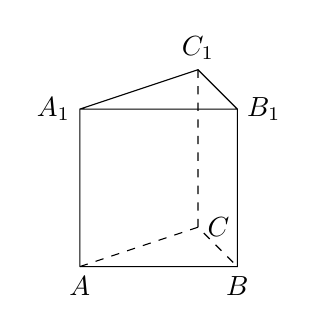
\begin{tikzpicture}[>=latex]
\draw (0,0) node [below] {$A$} coordinate (A);
\draw (2,0) node [below] {$B$} coordinate (B);
\draw (1.5,0.5) node [right] {$C$} coordinate (C);
\draw (A) ++ (0,2) node [left] {$A_1$} coordinate (A1);
\draw (B) ++ (0,2) node [right] {$B_1$} coordinate (B1);
\draw (C) ++ (0,2) node [above] {$C_1$} coordinate (C1);
\draw (A) -- (B) -- (B1) -- (A1) -- (A) (A1) -- (C1) -- (B1);
\draw [dashed] (A) -- (C) -- (B) (C) -- (C1);
\end{tikzpicture}
\end{center}
\item 如图, 直线$a$及直线$b$是异面直线, 直线$a$、$b$分别在两个平行平面$\alpha$和$\beta$上. 又设直线$l\perp a$, $l\perp b$. 求证: $l\perp \alpha$, $l\perp \beta$.
\begin{center}
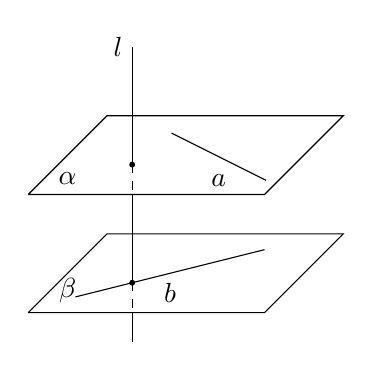
\begin{tikzpicture}[>=latex]
\draw (0,0) --++ (3,0) --++ (1,1) --++ (-3,0) --++ (-1,-1) coordinate (beta);
\draw (0,1.5) --++ (3,0) --++ (1,1) --++ (-3,0) --++ (-1,-1) coordinate (alpha);
\draw (alpha) ++ (0.5,0) node [above] {$\alpha$} (beta) ++ (0.5,0) node [above] {$\beta$};
\draw (0.6,0.2) coordinate (A) -- (3,0.8) coordinate (B);
\filldraw ($(A)!0.3!(B)$) circle (0.03) coordinate (C);
\filldraw (C) ++ (0,1.5) circle (0.03) coordinate (D);
\path [name path = CD] ($(C)!2!(D)$) -- ($(C)!-0.5!(D)$);
\path [name path = aboveline] (0,1.5) --++ (3,0);
\path [name path = belowline] (0,0) --++ (3,0);
\path [name intersections = {of = CD and aboveline, by = D1}];
\path [name intersections = {of = CD and belowline, by = C1}];
\draw ($(C)!2!(D)$) node [left] {$l$} -- (D) (D1) -- (C) (C1) -- ($(C)!-0.5!(D)$);
\draw [dashed] (D) -- (D1) (C) -- (C1);
\draw (D) ++ (0.5,0.4) --++ (1.2,-0.6);
\draw (D) ++ (1.1,0) node [below] {$a$};
\draw ($(A)!0.5!(B)$) node [below] {$b$};
\end{tikzpicture}
\end{center}
\item 如图, 设$\alpha$、$\beta$、$\gamma$三平面互相平行, 直线$a$与$b$分别交$\alpha$、$\beta$、$\gamma$于点$A$、$B$、$C$和点$D$、$E$、$F$. 求证: $ABBC=DEEF$.
\begin{center}
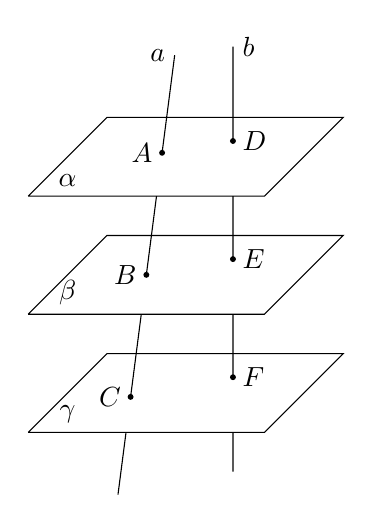
\begin{tikzpicture}[>=latex]
\draw (0,0) --++ (3,0) --++ (1,1) --++ (-3,0) --++ (-1,-1) ++ (0.5,0) node [above] {$\gamma$};
\draw (0,1.5) --++ (3,0) --++ (1,1) --++ (-3,0) --++ (-1,-1) ++ (0.5,0) node [above] {$\beta$};
\draw (0,3) --++ (3,0) --++ (1,1) --++ (-3,0) --++ (-1,-1) ++ (0.5,0) node [above] {$\alpha$};
\filldraw (2.6,2.2) circle (0.03) node [right] {$E$} coordinate (E);
\filldraw (1.5,2) circle (0.03) node [left] {$B$} coordinate (B);
\filldraw (E) ++ (0,1.5) circle (0.03) node [right] {$D$} coordinate (D);
\filldraw (E) ++ (0,-1.5) circle (0.03) node [right] {$F$} coordinate (F);
\filldraw (B) ++ (0.2,1.55) circle (0.03) node [left] {$A$} coordinate (A);
\filldraw (B) ++ (-0.2,-1.55) circle (0.03) node [left] {$C$} coordinate (C);
\path [name path = AC] ($(A)!-0.4!(C)$) node [left] {$a$} -- ($(A)!1.4!(C)$);
\path [name path = DF] ($(D)!-0.4!(F)$) node [right] {$b$} -- ($(D)!1.4!(F)$);
\path [name path = line1] (0,3) --++ (3,0);
\path [name path = line2] (0,1.5) --++ (3,0);
\path [name path = line3] (0,0) --++ (3,0);
\path [name intersections = {of = line1 and AC, by = A1}];
\path [name intersections = {of = line2 and AC, by = B1}];
\path [name intersections = {of = line3 and AC, by = C1}];
\path [name intersections = {of = line1 and DF, by = D1}];
\path [name intersections = {of = line2 and DF, by = E1}];
\path [name intersections = {of = line3 and DF, by = F1}];
\draw ($(A)!-0.4!(C)$) -- (A) (A1) -- (B) (B1) -- (C) (C1) -- ($(A)!1.4!(C)$);
\draw ($(D)!-0.4!(F)$) -- (D) (D1) -- (E) (E1) -- (F) (F1) -- ($(D)!1.4!(F)$);
\end{tikzpicture}
\end{center}
\item 在正方体$ABCD-A'B'C'D'$中, 平面$ABC'D'$与正方体的各个面所成的二面角的大小分别是多少?
\item 在$30^\circ$二面角的一个面内有一个点, 它到另一个面的距离是$10\text{cm}$. 求这个点到二面角的棱的距离.
\item 如图, 在四面体$ABCD$中, 已知$AB=AC=BD=CD=2$, $BC=2\sqrt 3$, 且$AD=1$. 试作出二面角$ABCD$的平面角, 并求它的度数.
\begin{center}
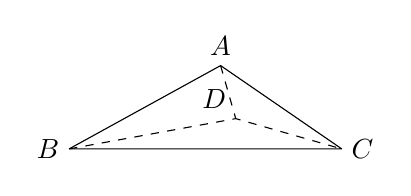
\begin{tikzpicture}[>=latex]
\draw ({sqrt(3)},0,0) node [right] {$C$} coordinate (C);
\draw ({-sqrt(3)},0,0) node [left] {$B$} coordinate (B);
\draw (0,0,-1) node [above left] {$D$} coordinate (D);
\draw (0,{sqrt(3)/2},{-1/2}) node [above] {$A$} coordinate (A);
\draw (B) -- (C) (B) -- (A) -- (C);
\draw [dashed] (A) -- (D) (B) -- (D) -- (C);
\end{tikzpicture}
\end{center}
\item 判断下列命题的真假, 并说明理由:\\
(1) 若平面$\alpha\perp$平面$\beta$, 平面$\beta\perp$平面$\gamma$, 则平面$\alpha\perp$平面$\gamma$;\\
(2) 若平面$\alpha\parallel$平面$\alpha_1$, 平面$\beta\parallel$平面$\beta_1$, 平面$\alpha\perp$平面$\beta$, 则平面$\alpha_1\perp$平面$\beta_1$.
\item 如图, 已知$AB$是平面$\alpha$的垂线, $AC$是平面$\alpha$的一条斜线, $CD$在$\alpha$上, 且垂直于$AC$. 求证: 平面$ABC\perp$平面$ACD$.
\begin{center}
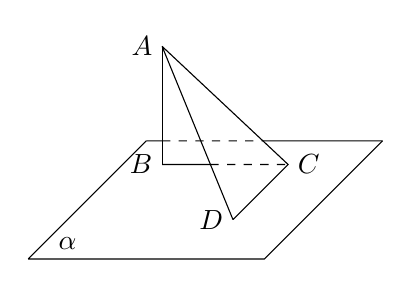
\begin{tikzpicture}[>=latex]
\draw (0,0) --++ (3,0) --++ (1.5,1.5) ++ (-3,0) --++ (-1.5,-1.5) ++ (0.5,0) node [above] {$\alpha$};
\draw (1.7,1.2) node [left] {$B$} coordinate (B) --++ (0,1.5) node [left] {$A$} coordinate (A);
\draw (B) ++ (1.6,0) node [right] {$C$} coordinate (C);
\draw (C) ++ (-0.7,-0.7) node [left] {$D$} coordinate (D);
\draw (A) -- (C) -- (D) (A) -- (D);
\path [name path = AD] (A) -- (D);
\path [name path = BC] (B) -- (C);
\path [name path = AB] (A) -- (B);
\path [name path = AC] (A) -- (C);
\path [name path = line] (1.5,1.5) --++ (3,0);
\path [name intersections = {of = AB and line, by = P}];
\path [name intersections = {of = AC and line, by = Q}];
\path [name intersections = {of = AD and BC, by = T}];
\draw (1.5,1.5) -- (P) (Q) -- (4.5,1.5) (B) -- (T);
\draw [dashed] (P) -- (Q) (T) -- (C);
\end{tikzpicture}
\end{center}
\item 已知平面$\alpha$、$\beta$、$\gamma$, 且$\alpha$及$\beta$均垂直于$\gamma$, 记$\alpha$与$\beta$的交线为$l$. 求证: $l$垂直于$\gamma$.
\item 假设$m$、$n$是两条相交直线, $l_1$、$l_2$是与$m$、$n$都垂直的两条直线, 但直线$l$至少与$m$、$n$中的一条不垂直. 求证:直线$l$与$l_1$、$l_2$所成的角相等.
\item 如图, 在四面体$VABC$中, 从顶点犞作平面$ABC$的垂线, 垂足$O$恰好落在$\triangle ABC$的中线$CD$上. 如果$VA=VB$, 能否判定$AC=BC$以及平面$VCD\perp$平面$VAB$?
\begin{center}
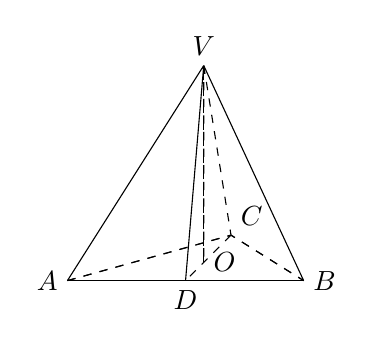
\begin{tikzpicture}[>=latex]
\draw (-1.5,0,0) node [left] {$A$} coordinate (A) -- (1.5,0,0) node [right] {$B$} coordinate (B);
\draw (0,0,0) node [below] {$D$} coordinate (D);
\draw (0,0,-1.5) node [above right] {$C$} coordinate (C);
\draw [dashed] (C) -- (D) (A) -- (C) -- (B);
\draw ($(D)!0.4!(C)$) node [right] {$O$} coordinate (O);
\draw [dashed] (O) --++ (0,2.5,0) node [above] {$V$} coordinate (V);
\draw (V) -- (A) (V) -- (B) (V) -- (D);
\draw [dashed] (V) -- (O) (V) -- (C) (A) -- (C) -- (B); 
\end{tikzpicture}
\end{center}
\item 证明: 三个两两垂直的平面的相应交线也两两垂直.
\item 自二面角内一点分别向两个面作垂线, 求证: 它们所成的角与二面角的平面角相等或互补.
\item 证明: 垂直于同一条直线的两个平面平行.
\item 已知一平面平行于两条异面直线, 一直线与两异面直线都垂直, 那么这个平面与这条直线的位置关系是\bracket{20}.
\fourch{平行}{垂直}{斜交}{不能确定}
\item 在棱长为$a$的正方体$ABCD-A_1B_1C_1D_1$中, 求:\\
(1) $D_1B_1$与$C_1C$之间的距离;\\
(2) $AC$与$D_1B_1$之间的距离.
\item 如图, 在四面体$ABCD$中, 已知所有棱长都为$a$. 求两异面直线$AB$与$CD$之间的距离.
\begin{center}
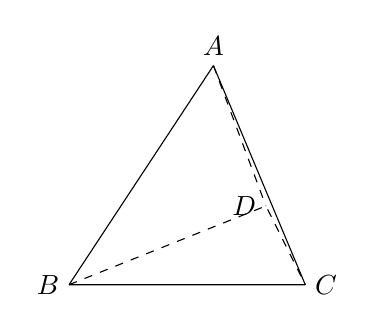
\begin{tikzpicture}[>=latex]
\draw (0,0,0) node [left] {$B$} coordinate (B);
\draw (3,0,0) node [right] {$C$} coordinate (C);
\draw (1.5,0,0) ++ (0,0,{-1.5*sqrt(3)}) node [left] {$D$} coordinate (D);
\draw (1.5,0,0) ++ (0,0,{-0.5*sqrt(3)}) ++ (0,{sqrt(6)},0) node [above] {$A$} coordinate (A); 
\draw (A) -- (B) (A) -- (C) (B) -- (C);
\draw [dashed] (B) -- (D) -- (C) (A) -- (D);
\end{tikzpicture}
\end{center}
\item 在$60^\circ$的二面角的棱上, 有两个点$A$、$B$, $AC$、$BD$分别是这个二面角的两个面上垂直于$AB$的线段. 已知$AB=4\text{cm}$, $AC=6\text{cm}$, $BD=8\text{cm}$. 求$CD$的长.
\item 若两异面直线$a$、$b$所成的角为$70^\circ$, 过空间内一点$P$作与直线$a$、$b$所成角均是$70^\circ$的直线$l$, 则所作直线$l$的条数为\bracket{20}.
\fourch{$1$}{$2$}{$3$}{$4$}
\item 如果两个平面分别垂直于两条异面直线中的一条, 求证: 这两个平面的交线与这两条异面直线的公垂线平行或重合.
\item 在直二面角的棱上有$A$、$B$两点, $AC$和$BD$分别在两个面上, 并且都垂直于棱$A$, 若$AB=8\text{cm}$, $AC=6\text{cm}$, $BD=24\text{cm}$, 求$CD$的长及$AB$和$CD$之间的距离.
\item 如图, 在长方体$ABCD-A_1B_1C_1D_1$中, $AB=a$, $BC=b$, $AA_1=c$. 求异面直线$B_1B$与$AC_1$之间的距离.
\begin{center}
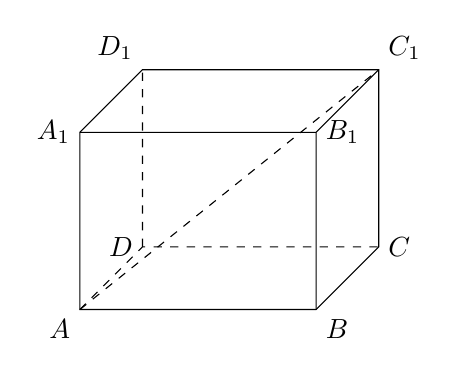
\begin{tikzpicture}[>=latex,scale = 1.5]
\draw (0,0) node [below left] {$A$} coordinate (A) --++ (2,0) node [below right] {$B$} coordinate (B) --++ (45:{1.5/2}) node [right] {$C$} coordinate (C)
--++ (0,1.5) node [above right] {$C_1$} coordinate (C1)
--++ (-2,0) node [above left] {$D_1$} coordinate (D1) --++ (225:{1.5/2}) node [left] {$A_1$} coordinate (A1) -- cycle;
\draw (A) ++ (2,1.5) node [right] {$B_1$} coordinate (B1) -- (B) (B1) --++ (45:{1.5/2}) (B1) --++ (-2,0);
\draw [dashed] (A) --++ (45:{1.5/2}) node [left] {$D$} coordinate (D) --++ (2,0) (D) --++ (0,1.5);
\draw [dashed] (A) -- (C1);
\end{tikzpicture}
\end{center}
\item 如图, 已知正方体$ABCD-A_1B_1C_1D_1$的棱长为$1$. 求异面直线$A_1B$与$B_1D_1$之间的距离.
\begin{center}
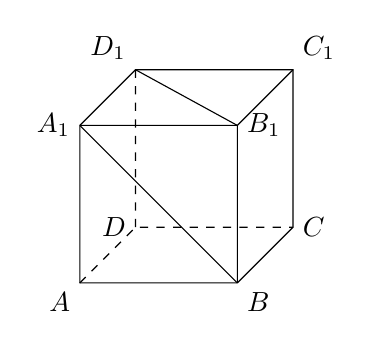
\begin{tikzpicture}[>=latex]
\draw (0,0) node [below left] {$A$} coordinate (A) --++ (2,0) node [below right] {$B$} coordinate (B) --++ (45:{2/2}) node [right] {$C$} coordinate (C)
--++ (0,2) node [above right] {$C_1$} coordinate (C1)
--++ (-2,0) node [above left] {$D_1$} coordinate (D1) --++ (225:{2/2}) node [left] {$A_1$} coordinate (A1) -- cycle;
\draw (A) ++ (2,2) node [right] {$B_1$} coordinate (B1) -- (B) (B1) --++ (45:{2/2}) (B1) --++ (-2,0);
\draw [dashed] (A) --++ (45:{2/2}) node [left] {$D$} coordinate (D) --++ (2,0) (D) --++ (0,2);
\draw (A1) -- (B) (B1) -- (D1);
\end{tikzpicture}
\end{center}
\item 若圆柱的底面半径是$1$, 母线长为$2$, 则这个圆柱的体积是\blank{50}.
\item 若一个圆柱的侧面积是$4\pi$, 高为$1$, 则这个圆柱的体积是\blank{50}.
\item 若正六棱柱的高为$4$, 底面边长为$2$, 则这个正六棱柱的体积是\blank{50}.
\item 将一个棱长为$a$的正方体切成$27$个全等的小正方体, 其表面积增加了\blank{50}.
\item 已知侧面都是矩形的四棱柱, 侧棱长为$5$, 底面是边长为$2$的菱形, 则这个棱柱的侧面积是\blank{50}.
\item 在正四棱柱$ABCD-A_1B_1C_1D_1$中, 若$AA_1=2AB$, 则异面直线$CD$与$AC_1$所成角的大小为\blank{50}.
\item 在正方体$ABCD-A_1B_1C_1D_1$中, 若$E$是$BC_1$的中点, 则直线$DE$与平面$ABCD$所成角的大小为\blank{50}.
\item 已知三棱柱$ABCA_1B_1C_1$的三个侧面均是矩形, 求证:它的任意两个侧面的面积之和大于第三个侧面的面积.
\item 已知长方体$ABCD-A_1B_1C_1D_1$的对角线$AC_1$的长是$l$, 且直线$AC_1$与长方体经过点$A$的三个面所成角分别是$\alpha$、$\beta$、$\gamma$. 求此长方体的体积.
\item 如图, 设圆柱有一个内接棱柱(即棱柱的侧棱都是圆柱的母线, 棱柱的两个底面分别在圆柱的两个底面内). 已知圆柱的体积是$4\sqrt 3\pi$, 棱柱的底面是边长为$2$的正三角形. 求棱柱的体积.
\begin{center}
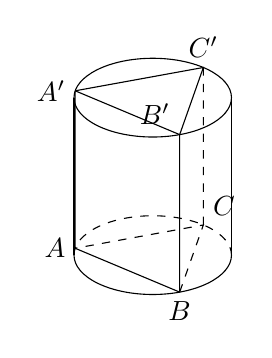
\begin{tikzpicture}[>=latex]
\draw (0,0) ellipse (1 and 0.5);
\draw (-1,-2) arc (180:360:1 and 0.5);
\draw [dashed] (-1,-2) arc (180:0:1 and 0.5);
\draw (0,-2) ++ ({cos(50)},{0.5*sin(50)}) node [above right] {$C$} coordinate (C);
\draw (0,-2) ++ ({cos(170)},{0.5*sin(170)}) node [left] {$A$} coordinate (A);
\draw (0,-2) ++ ({cos(290)},{0.5*sin(290)}) node [below] {$B$} coordinate (B);
\draw (A) ++ (0,2) node [left] {$A'$} coordinate (A1);
\draw (B) ++ (0,2) node [above left] {$B'$} coordinate (B1);
\draw (C) ++ (0,2) node [above] {$C'$} coordinate (C1);
\draw (A1) -- (B1) -- (C1) -- (A1);
\draw (A) -- (A1) (B) -- (B1) (A) -- (B);
\draw [dashed] (B) -- (C) -- (A) (C) -- (C1);
\draw (-1,-2) -- (-1,0) (1,-2) -- (1,0);
\end{tikzpicture}
\end{center}
\item 如图, 一个直三棱柱形容器中盛有水, 且侧棱$AA_1=8$. 当侧面$AA_1B_1B$水平放置时, 液面恰好过$AC$、$BC$、$A_1C_1$、$B_1C_1$的中点. 当底面$ABC$水平放置时, 液面高为多少? 
\begin{center}
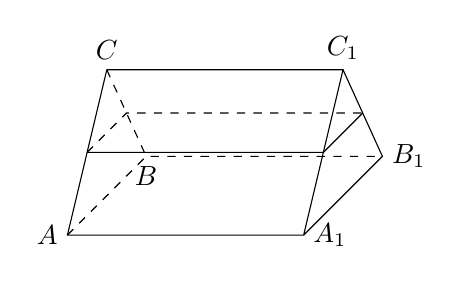
\begin{tikzpicture}[>=latex]
\draw (0,0) node [left] {$A$} coordinate (A);
\draw (1,1) node [below] {$B$} coordinate (B);
\draw (0.5,2.1) node [above] {$C$} coordinate (C);
\draw (A) ++ (3,0) node [right] {$A_1$} coordinate (A1);
\draw (B) ++ (3,0) node [right] {$B_1$} coordinate (B1);
\draw (C) ++ (3,0) node [above] {$C_1$} coordinate (C1);
\draw (C) -- (C1) -- (A1) -- (A) -- (C) (A1) -- (B1) -- (C1);
\draw [dashed] (C) -- (B) -- (B1) (A) -- (B);
\draw ($(A)!0.5!(C)$) --++ (3,0) --++ (0.5,0.5);
\draw [dashed] ($(A)!0.5!(C)$) --++ (0.5,0.5) --++ (3,0);
\end{tikzpicture}
\end{center}
\item 已知一个正三棱锥的底面边长为$6$, 侧棱长为$\sqrt 15$. 求这个三棱锥的体积.
\item 如图, 已知三棱锥$PABC$中, $PA$垂直于平面$ABC$,$ AB\perp BC$, $PA=4$, $AB=3$, $AC=5$.
\begin{center}
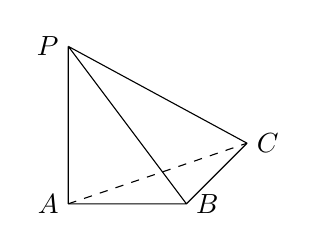
\begin{tikzpicture}[>=latex,scale = 0.5]
\draw (0,0,0) node [left] {$A$} coordinate (A);
\draw (A) ++ (0,4,0) node [left] {$P$} coordinate (P);
\draw (A) ++ (3,0,0) node [right] {$B$} coordinate (B);
\draw (B) ++ (0,0,-4) node [right] {$C$} coordinate (C);
\draw (A) -- (B) -- (C) (P) -- (A) (P) -- (C) (P) -- (B);
\draw [dashed] (A) -- (C);
\end{tikzpicture}
\end{center}
(1) 求点$A$到平面$PBC$的距离;\\
(2) 求三棱锥$PABC$的表面积.
\item 把边长为$1$的正方形$ABCD$沿对角线$AC$折起, 使(折叠后的)$A$、$B'$、$C$、$D$四点为顶点的三棱锥体积最大. 求此三棱锥的表面积.
\begin{center}
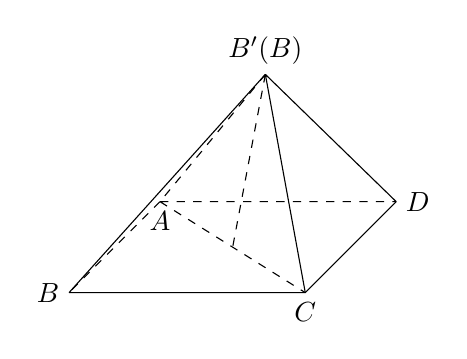
\begin{tikzpicture}[>=latex]
\draw (0,0,0) node [left] {$B$} coordinate (B);
\draw (3,0,0) node [below] {$C$} coordinate (C);
\draw (3,0,-3) node [right] {$D$} coordinate (D);
\draw (0,0,-3) node [below] {$A$} coordinate (A);
\draw (B) -- (C) -- (D);
\draw [dashed] (A) -- (B) (A) -- (C) (A) -- (D);
\draw (1.8,{sqrt(2*pow(1.5,2)-2*pow(0.3,2))},-1.8) node [above] {$B'(B)$} coordinate (B1);
\draw (B) -- (B1) (B1) -- (C) (B1) -- (D);
\draw [dashed] (B1) -- (A) (B1) -- ($(A)!0.5!(C)$);
\end{tikzpicture}
\end{center}
\item 棱锥被平行于底面的平面所截, 当截面分别平分棱锥的高与体积时, 相应的截面面积分别为$S_1$、$S_2$. 求证: $S_1<S_2$.
\item 若圆锥的底面半径为$1$, 高为$\sqrt 3$, 求圆锥的表面积.
\item 把一个圆锥截成圆台, 已知圆台的上、下底面半径的比为$1: 4$, 母线(原圆锥母线在圆台中的部分)长为$10\text{cm}$. 求原圆锥的母线长.
\item 已知圆锥的底面半径为$3$, 沿该圆锥的母线把侧面展开后可得到圆心角为$\dfrac{2\pi}3$的扇形. 求该圆锥的高.
\item 用一个平面去截正方体, 得到一个三棱锥, 截得的三棱锥中, 除了截面外另三个面的面积分别为$S_1$、$S_2$、$S_3$. 求这个三棱锥的体积.
\item 在三棱锥$PABC$中, 已知$PA=PB=PC=1$, $AB=\sqrt 2$, $BC=1$, $AC=\sqrt 3$. 求该三棱锥底面$ABC$上的高与三棱锥的体积.
\item 用过圆柱和圆锥的轴的平面截这两个几何体, 分别得到边长为$2$的正方形和正三角形, 求圆柱和圆锥的表面积之比.
\item 已知圆锥底面的半径为$10$, 母线长为$60$. 求底面圆周上一点$B$沿侧面绕两周回到点$B$的最短距离.
\item 设圆台的母线长为$l$, 上、下底面的半径分别为$r'$、$r$. 试用$r'$、$r$和$l$表示圆台的侧面积.
\item 如图, 以正方体$ABCD-A_1B_1C_1D_1$六个面的中心为顶点所构成的多面体有多少条棱和多少个面?  设正方体的棱长为$1$, 这个多面体的表面积和体积是多少? 
\begin{center}
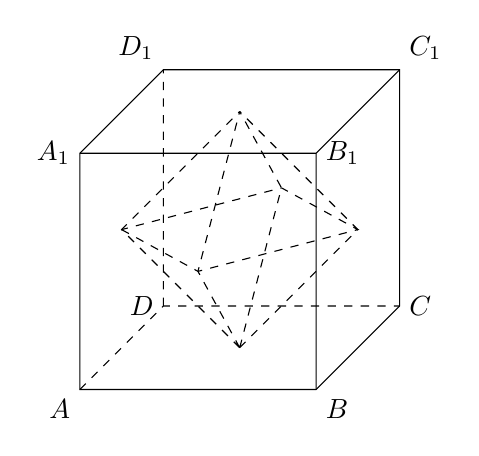
\begin{tikzpicture}[>=latex]
\draw (0,0) node [below left] {$A$} coordinate (A) --++ (3,0) node [below right] {$B$} coordinate (B) --++ (45:{3/2}) node [right] {$C$} coordinate (C)
--++ (0,3) node [above right] {$C_1$} coordinate (C1)
--++ (-3,0) node [above left] {$D_1$} coordinate (D1) --++ (225:{3/2}) node [left] {$A_1$} coordinate (A1) -- cycle;
\draw (A) ++ (3,3) node [right] {$B_1$} coordinate (B1) -- (B) (B1) --++ (45:{3/2}) (B1) --++ (-3,0);
\draw [dashed] (A) --++ (45:{3/2}) node [left] {$D$} coordinate (D) --++ (3,0) (D) --++ (0,3);
\draw ($(A)!0.5!(D1)$) coordinate (P);
\draw ($(B)!0.5!(A1)$) coordinate (Q);
\draw ($(C)!0.5!(B1)$) coordinate (R);
\draw ($(D)!0.5!(C1)$) coordinate (S);
\draw ($(A)!0.5!(C)$) coordinate (X);
\draw ($(A1)!0.5!(C1)$) coordinate (Y);
\draw [dashed] (P) -- (Q) -- (R) -- (S) -- (P);
\draw [dashed] (X) -- (P) -- (Y) (X) -- (Q) -- (Y) (X) -- (R) -- (Y) (X) -- (S) -- (Y);
\end{tikzpicture}
\end{center}
\item 如图, 设$E$、$F$、$G$分别是正方体$ABCD-A_1B_1C_1D_1$的共点的三条棱$A_1B_1$、$B_1B$、$B_1C_1$的中点, 过这三个点的平面截正方体得到的一个``角''是四面体$B_1EFG$. 设正方体的棱长为$1$.
\begin{center}
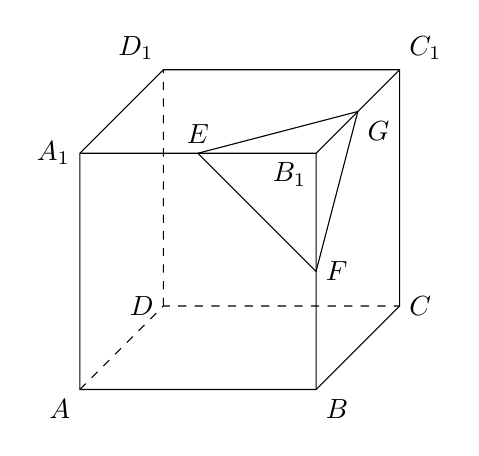
\begin{tikzpicture}[>=latex]
\draw (0,0) node [below left] {$A$} coordinate (A) --++ (3,0) node [below right] {$B$} coordinate (B) --++ (45:{3/2}) node [right] {$C$} coordinate (C)
--++ (0,3) node [above right] {$C_1$} coordinate (C1)
--++ (-3,0) node [above left] {$D_1$} coordinate (D1) --++ (225:{3/2}) node [left] {$A_1$} coordinate (A1) -- cycle;
\draw (A) ++ (3,3) node [below left] {$B_1$} coordinate (B1) -- (B) (B1) --++ (45:{3/2}) (B1) --++ (-3,0);
\draw [dashed] (A) --++ (45:{3/2}) node [left] {$D$} coordinate (D) --++ (3,0) (D) --++ (0,3);
\draw ($(B1)!0.5!(A1)$) node [above] {$E$} coordinate (E);
\draw ($(B)!0.5!(B1)$) node [right] {$F$} coordinate (F);
\draw ($(B1)!0.5!(C1)$) node [below right] {$G$} coordinate (G);
\draw (E) -- (F) -- (G) -- cycle;
\end{tikzpicture}
\end{center}
(1) 求证:四面体$B_1EFG$是以$B_1$为顶点、以$EFG$为底面的正三棱锥;\\
(2) 在四面体$B_1EFG$中, 求顶点$B_1$到底面$EFG$的距离;\\
(3) 如果将正方体按照题设的方法截去八个``角'', 那么剩余的多面体有几个顶点、几条棱、几个面? 并求这个剩余多面体的表面积与体积.
\item 在如图所示的多面体中, 已知$ABCD$为矩形, $ABFE$和$DCFE$为全等的等腰梯形, $AB=4$, $BC=AE=EF=2$. 求此多面体的表面积与体积.
\begin{center}
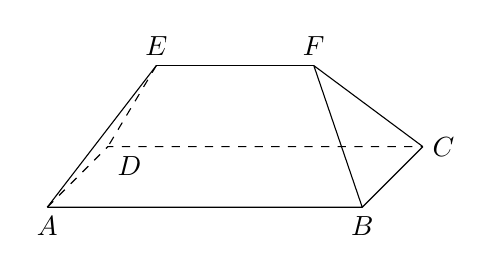
\begin{tikzpicture}[>=latex]
\draw (0,0,0) node [below] {$A$} coordinate (A);
\draw (4,0,0) node [below] {$B$} coordinate (B);
\draw (0,0,-2) node [below right] {$D$} coordinate (D);
\draw (4,0,-2) node [right] {$C$} coordinate (C);
\draw (1,{sqrt(2)},-1) node [above] {$E$} coordinate (E);
\draw (E) --++ (2,0,0) node [above] {$F$} coordinate (F);
\draw (A) -- (B) -- (C) (A) -- (E) (F) -- (B) (F) -- (C);
\draw [dashed] (E) -- (D) (A) -- (D) -- (C);
\end{tikzpicture}
\end{center}
\item 一个直角三角形有一个$\dfrac\pi 6$的内角, 这个内角所对直角边的长度为$1$. 把这个三角形绕其斜边旋转一周, 求所得旋转体的表面积与体积.
\item 如图, 给定一个正方体形状的土豆块, 只切一刀, 可以得到下面哪些类型的多面体? 
\begin{center}
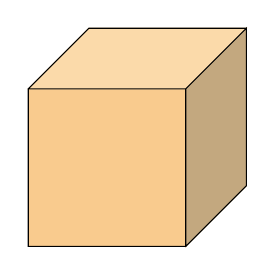
\begin{tikzpicture}[>=latex]
\definecolor{frontcolor}{RGB}{249, 203, 142}
\filldraw [frontcolor] (0,0,0) rectangle (2,2,0);
\definecolor{rightcolor}{RGB}{195, 168, 127}
\filldraw [rightcolor] (2,0,0)  -- (2,0,-2) -- (2,2,-2) -- (2,2,0) -- cycle;
\definecolor{abovecolor}{RGB}{251, 218, 170}
\filldraw [abovecolor] (0,2,0) -- (2,2,0) -- (2,2,-2) -- (0,2,-2) -- cycle;
\draw (0,0,0) rectangle (2,2,0) (2,0,0)  -- (2,0,-2) -- (2,2,-2) -- (2,2,0) (0,2,0) -- (0,2,-2) -- (2,2,-2);
\end{tikzpicture}
\end{center}
\textcircled{1} 四面体; \textcircled{2} 四棱锥; \textcircled{3} 四棱柱; \textcircled{4} 五棱锥; \textcircled{5} 五棱柱; \textcircled{6} 六棱锥; \textcircled{7} 七面体. \blank{100}(找出可能的结果, 并将序号填在横线上).
\item 如图, 有两张全等的正三角形纸片, 按照下面两种方法分别将它们剪拼成一个三棱锥和一个三棱柱. 试比较这两个多面体的体积的大小.
\begin{center}
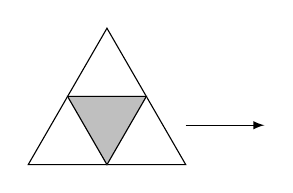
\begin{tikzpicture}[>=latex]
\draw (0,0) -- (2,0) -- (60:2) -- cycle;
\filldraw [gray!50] (60:1) --++ (1,0) -- (1,0) -- cycle;
\draw (60:1) --++ (1,0) -- (1,0) -- cycle;
\draw [->] (2,0.5) -- (3,0.5);
\end{tikzpicture}
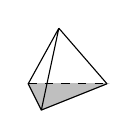
\begin{tikzpicture}[>=latex]
\draw (0,0,0) coordinate (A)  (1,0,0) coordinate (B)  (0.5,0,{0.5*sqrt(3)}) coordinate (C) (C) ++ (0,0,{-0.5*sqrt(3)/3*2}) ++ (0,{sqrt(6)/3},0) coordinate (D);
\filldraw [gray!50] (A) -- (C) -- (B) -- cycle;
\draw (D) -- (A) (D) -- (B) (D) -- (C) (A) -- (C) -- (B);
\draw [dashed] (A) -- (B);
\end{tikzpicture}
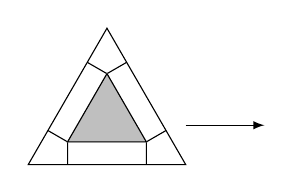
\begin{tikzpicture}[>=latex]
\draw (0,0) -- (2,0) -- (60:2) -- cycle;
\draw (30:{1/sqrt(3)}) coordinate (A);
\draw (A) ++ (1,0) coordinate (B);
\draw (A) ++ (60:1) coordinate (C);
\draw (A) --++ (0,{-0.5/sqrt(3)}) (A) --++ (150:{0.5/sqrt(3)});
\draw (B) --++ (270:{0.5/sqrt(3)}) (B) --++ (30:{0.5/sqrt(3)});
\draw (C) --++ (30:{0.5/sqrt(3)}) (C) --++ (150:{0.5/sqrt(3)});
\filldraw [gray!50] (A) -- (B) -- (C) -- cycle;
\draw (A) -- (B) -- (C) -- cycle;
\draw [->] (2,0.5) -- (3,0.5);
\end{tikzpicture}
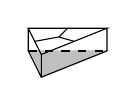
\begin{tikzpicture}[>=latex]
\draw (0,0,0) coordinate (A)  (1,0,0) coordinate (B)  (0.5,0,{0.5*sqrt(3)}) coordinate (C);
\filldraw [gray!50] (A) -- (C) -- (B) -- cycle;
\draw (A) ++ (0,{0.5/sqrt(3)}) coordinate (A1) (B) ++ (0,{0.5/sqrt(3)}) coordinate (B1) (C) ++ (0,{0.5/sqrt(3)}) coordinate (C1);
\draw (A1) -- (B1) -- (C1) -- cycle;
\draw (A) -- (A1) (B) -- (B1) (C) -- (C1) (A) -- (C) -- (B);
\draw [dashed] (A) -- (B);
\draw (C1) ++ (0,0,{-0.5*sqrt(3)/3*2}) coordinate (D);
\draw ($(A1)!0.5!(B1)$) -- (D) ($(C1)!0.5!(B1)$) -- (D) ($(C1)!0.5!(A1)$) -- (D);
\end{tikzpicture}
\end{center}
\item 若一个球的体积是$\dfrac 43\pi$, 则这个球的表面积是\blank{50}.
\item 若用与球心距离为$1$的平面截球体所得的圆面半径为$3$, 则球的体积为\blank{50}.
\item 若平面$\alpha$截球$O$所得圆的半径为$1$, 球的表面积是$12\pi$, 则球心$O$到平面$\alpha$的距离为\blank{50}.
\item 已知两个球的表面积之差为$48\pi$, 它们的大圆周长之和为$12\pi$, 则这两个球的半径之差为\blank{50}.
\item 已知正三角形$ABC$的三个顶点都在半径为$2$的球面上, 球心$O$到平面$ABC$的距离为$1$, $E$是线段$AB$的中点, 过点$E$作球$O$的截面, 则截面面积的最小值是\blank{50}.
\item 已知过球面上$A$、$B$、$C$三点的截面和球心的距离等于球半径的一半, 且$AB=BC=CA=2$. 求截面的面积.
\item 已知三棱柱$ABC-A_1B_1C_1$的$6$个顶点都在球$O$的球面上, 且$AB=3, AC=4$, $AB\perp AC$, $AA_1=12$. 求球$O$的半径.
\item 如图为一个用鲜花做成的花柱, 它的下面是一个直径为$1\text{m}$、高为$3\text{m}$的圆柱形物体, 上面是一个半球形体. 如果每平方米大约需要鲜花$120$朵, 那么装饰这个花柱大约需要多少朵鲜花?
\begin{center}
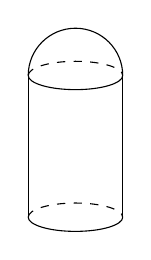
\begin{tikzpicture}[>=latex,scale = 0.6]
\draw (-1,0) arc (180:360:1 and 0.3);
\draw (-1,3) arc (180:360:1 and 0.3);
\draw [dashed] (-1,0) arc (180:0:1 and 0.3);
\draw [dashed] (-1,3) arc (180:0:1 and 0.3);
\draw (-1,3) arc (180:0:1);
\draw (-1,0) -- (-1,3) (1,0) -- (1,3);
\end{tikzpicture}
\end{center}
\item 如图, 半径为$R$的球$O$中有一内接圆柱, 当圆柱的侧面积最大时, 求球的表面积与该圆柱的侧面积之差.
\begin{center}
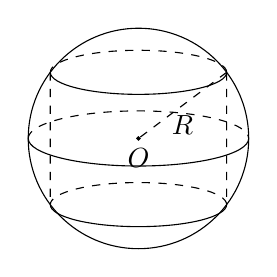
\begin{tikzpicture}[>=latex,scale = 0.7]
\draw (0,0) circle (2);
\filldraw (0,0) circle (0.03) node [below] {$O$} coordinate (O);
\draw [dashed] (1.6,1.2) coordinate (P) -- (O);
\draw (-2,0) arc (180:360:2 and 0.5);
\draw (0.8,0.6) node [below] {$R$};
\draw [dashed] (-2,0) arc (180:0:2 and 0.5);
\draw [dashed] (P) -- (1.6,-1.2) (-1.6,1.2) -- (-1.6,-1.2);
\draw (P) arc (0:-180:1.6 and 0.4);
\draw (P) ++ (0,-2.4) arc (0:-180:1.6 and 0.4);
\draw [dashed] (P) arc (0:180:1.6 and 0.4);
\draw [dashed] (P) ++ (0,-2.4) arc (0:180:1.6 and 0.4);
\end{tikzpicture}
\end{center}
\item 判断下列事件中, 哪些是确定的事件, 哪些是不确定的事件?\\
(1) 在空地上抛一石块, 石块会下落;\\
(2) 明天上午八时到九时之间, 你会接到一个推销电话;\\
(3) 买一张福利彩票, 会中奖.
\item 抛掷$100$枚同一类型且质地均匀的硬币, 下面的陈述哪些是正确的, 哪些是错误的?\\
(1) 全部出现正面向上是不可能的;\\
(2) 至少有$1$枚出现正面向上是必然的;\\
(3) 出现$50$枚正面向上、$50$枚正面向下是不确定的.
\item 从装有红、白、黑三种颜色的小球各$1$个的袋子中任取$2$个小球, 写出这个随机试验的样本空间.
\item ``一名学生一次掷$3$颗骰子, $3$颗都掷得点数$6$''的事件是\bracket{20}.
\twoch{不可能事件}{必然事件}{可能性较大的随机事件}{可能性较小的随机事件}
\item 下列哪些是不确定的事件?\\
(1) 学生甲明天竞选班长成功;\\
(2) 两支足球队明天比赛, 主场队取胜;\\
(3) 若集合$A$、$B$、$C$满足$A\subseteq B\subseteq C$, 则$A\subseteq C$.
\item 一个口袋中有大小与质地相同的$1$个白球、$2$个黑球、$3$个红球, 从中任取$2$个球, 观察球的颜色. 写出样本空间及与下列事件相应的基本事件子集:\\
(1) 含有白球;\\
(2) 至少含有$1$个黑球.
\item 两个男生、两个女生随机站一排,\\
(1) 写出样本空间;\\
(2) 写出每个人的相邻之人总是异性这个事件所对应的子集;\\
(3) 写出每个人的相邻之人至少有一个异性这个事件所对应的子集.
\item 从$1$、$2$、$3$、$4$、$5$中任取$3$个不同的数, 求这$3$个数构成一组勾股数(或者说恰为一个直角三角形的三条边长)的概率.
\item 如果将一枚质地均匀的硬币连续抛掷$100$次, 那么第$99$次出现反面朝上的概率是\bracket{20}.
\fourch{$\dfrac 1{100}$}{$\dfrac{99}{100}$}{$\dfrac{1}{99}$}{$\dfrac 12$}
\item 在分别写有数字$0$、$1$、$2$、$3$、$4$、$5$、$6$、$7$、$8$、$9$的$10$张一样的卡片中随机抽取$1$张. 设事件$A$: 出现奇数, 事件$B$: 出现偶数, 事件$C$: 大于$4$. 写出下列事件对应的集合:\\
(1) $A$、$C$同时发生;\\
(2) $B$、$C$至少有一个发生;\\
(3) $A$、$B$同时发生.
\item 掷一颗骰子, 设事件$A$: 落地时向上的点数是奇数, 事件$B$: 落地时向上的点数是偶数, 事件$C$: 落地时向上的点数是$3$的倍数, 事件$D$: 落地时向上的点数是$4$. 则下列每对事件中, 不是互斥事件的为\bracket{20}.
\fourch{$A$与$B$}{$B$与$C$}{$A$与$D$}{$C$与$D$}
\item 如图, 靶子由一个中心圆面$\text{I}$$\text{I}$同心的圆环$\text{II}$、$\text{III}$构成, 射手命中$\text{I}$、$\text{II}$及$\text{III}$的概率分别为$0.35$、$0.30$及$0.25$. 求不命中靶的概率.
\begin{center}
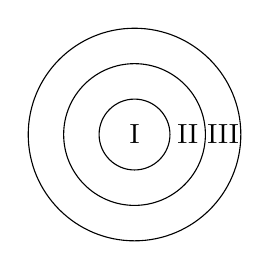
\begin{tikzpicture}[>=latex,scale = 1.5]
\draw (0,0) circle (0.3) node {\text{I}};
\draw (0,0) circle (0.6) (0.45,0) node {\text{II}};
\draw (0,0) circle (0.9) (0.75,0) node {\text{III}};
\end{tikzpicture}
\end{center}
\item 盒子里装有大小与质地相同的红球与白球, 从中任取$3$个球.设事件$A$表示``$3$个球中有$1$个红球、$2$个白球'', 事件$B$表示``3个球中有$2$个红球、$1$个白球''. 已知$P(A)=\dfrac{3}{10}$, $P(B)=\dfrac 12$. 求``$3$个球中既有红球又有白球''的概率.
\item 已知$4$张奖券中只有$1$张能中奖, 现分别由$4$名学生依次抽取(抽出后不放回), 他们的中奖概率是否一样? 为什么?
\item 已知$5$件产品中有$2$件次品、$3$件合格品, 从这$5$件产品中任取$2$件, 求:\\
(1) 恰有$1$件次品的概率;\\
(2) $2$件都是合格品的概率.
\item 已知关于$x$的一元二次方程$x^2-ax+3=0$, 其中$a$是掷一颗骰子得到的点数. 求下列事件的概率:\\
(1) 方程有两个不相等的实根;\\
(2) $x=3$是方程的根;\\
(3) 方程存在正根.
\item 已知事件$A$与$B$互斥, 它们都不发生的概率为$\dfrac 25$, 且$P(A)=2P(B)$. 求$P(\overline A)$.
\item 袋中有大小与质地相同的$12$个小球, 分别为红球、黑球、黄球、绿球, 从中任取$1$个球, 得到红球的概率是$\dfrac 13$, 得到黑球或黄球的概率是$\dfrac{5}{12}$, 得到黄球或绿球的概率是$\dfrac{5}{12}$. 试求得到黑球、黄球、绿球的概率各是多少.
\item 一家保险公司想了解汽车的挡风玻璃在一年时间内破碎的概率, 于是调查了$20000$辆汽车, 发现在一年时间内共有$600$辆汽车的挡风玻璃破碎. 求一辆汽车在一年时间内挡风玻璃破碎的经验概率.
\item 为了估计装有$5$个白球和若干个红球(每个球的大小与质地相同)的袋中红球的个数, 在不将袋中球倒出来的情况下, 分$20$个小组进行摸球试验. 每组两人, 其中一位学生摸球, 另一位学生记录所摸球的颜色, 再将球放回袋中摇匀. 每一组各做$400$次试验, 汇总后, 摸到红球的次数为$6000$次.\\
(1) 估计从袋中任意摸出$1$个球, 恰好是红球的概率;\\
(2) 估计袋中红球的个数.
\item 甲盒中有红、黑、白三种颜色的球各$3$个, 乙盒中有黄、黑、白三种颜色的球各$2$个, 各个球的大小与质地相同. 从两个盒子中各取$1$个球.\\
(1) 求取出的$2$个球颜色不同的概率;\\
(2)设计一个随机试验, 计算(1)中取出的$2$个球是不同颜色的经验概率.
\item 上数学课时, 教师给班里学生出了两道选择题, 教师预估做对第一道题的概率为$0.80$, 做对两道题的概率为$0.60$, 假设这两道题是独立的, 问:预估做对第二道题的概率是多少? 
\item 某人有$4$把钥匙, 其中$2$把能打开门. 现随机地取$1$把钥匙开门.\\
(1) 如果将不能开门的钥匙立即扔掉, 求第二次才能打开门的概率;\\
(2) 如果试过的钥匙不扔掉, 求第二次才能打开门的概率.
\item 如果$A$、$B$是独立事件, $\overline A$、$\overline B$分别是$A$、$B$的对立事件, 那么以下等式不一定成立的是\bracket{20}.
\twoch{$P(A\cap B)=P(A)P(B)$}{$P(\overline A\cap B)=P(\overline A)P(B)$}{$P(A\cup B)=P(A)+P(B)$}{$P(\overline A\cap \overline B)=[1-P(A)][1-P(B)]$}
\item 如果从甲口袋中摸出一个红球的概率是$\dfrac 13$, 从乙口袋中摸出一个红球的概率是$\dfrac 12$, 求下面四个事件的概率:\\
(1) $2$个球不都是红球;\\
(2) $2$个球都是红球;\\
(3) 至少有$1$个红球;\\
(4) $2$个球中恰好有$1$个红球.
\item 设甲和乙两射手独立地射击同一目标, 他们的命中率分别为$0.95$和$0.90$. 求:\\
(1) 在一次射击中, 目标被击中的概率;\\
(2) 目标只被甲击中的概率.
\item 把分奖金问题的三局两胜改为五局三胜, 问:\\
(1) 在比分是$2: 0$的情况下, 怎么分奖金公平?\\
(2) 在比分是$1: 0$的情况下, 怎么分奖金公平? 
\item 某农业研究人员为考察三个品种的小麦发芽率, 从中选取麦种若干, 经检测得到数据如下表所示. 在这个问题中, 总体和样本分别是什么? 样本量是多少?
\begin{center}
\begin{tabular}{|c|c|c|}
\hline
品种 & 麦种数 & 发芽数 \\ \hline
$A$ & $100$ & $92$ \\ \hline
$B$ & $200$ & $189$ \\ \hline
$C$ & $200$ & $182$ \\ \hline
\end{tabular}
\end{center}
\item 小王和小张计划调查上海市新生儿的性别情况. 小王调查了最近一个月在$A$医院出生的$320$名新生儿, 其中有$156$名女孩, 小王由此推断: 上海市新生儿男女比例基本均衡. 小张的姐姐在$B$医院待产, 她告诉小张最近一周在$B$医院出生的$18$名新生儿中有$13$名女孩, 小张由此推断: 上海市新生儿男女比例严重失调. 考虑下面的问题:\\
(1) 在上面的统计活动中, 总体和样本分别是什么?\\
(2) 你同意小王和小张的推断吗?  请说一说你的理由.\\
(3) 你认为是否可以用上面的样本来推断上海市新生儿的男女比例? 请说一说你的理由. 
\item 测量队要测量一个池塘的平均深度, 选择了池塘的$150$个不同的位置进行测量, 得到了$150$个数据, 然后用这$150$个数据的平均数来估计池塘的平均深度. 在这项统计活动中, 总体和样本分别是什么?
\item 在某校高一年级的期中数学测验中, 很多学生在解决一道应用题时都出现了错误. 教师在试卷分析时说: ``看起来, 我们高一(3)班的同学解决应用问题比较薄弱. ''请你从统计的角度来讨论下面的问题:\\
(1) 在这个情境中, 总体和样本分别是什么?\\
(2) 你同意教师的说法吗? 请说明理由.
\item 统计在日常生活中有大量的应用, 请收集$2$至$3$个统计案例, 并说明其总体和样本分别是什么.
\item 小明为了解自己每天花在体育锻炼上的时间(单位: $\text{min}$), 连续记录了$10$天的数据, 它们分别是: $68$、$34$、$70$、$45$、$74$、$126$、$108$、$66$、$36$、$72$. 在这个问题中, 总体和样本分别是什么? 
\item 回答以下问题需要获得的数据是观测数据还是实验数据?\\
(1) 本班级每名学生对数学中某个知识点的掌握程度如何?\\
(2) 消费者对于某品牌饮料的喜爱程度如何?\\
(3) 户外运动时间是否会影响青少年的视力?
\item 试调查去年我国有多少所普通高中学校, 共有多少名在校学生.
\item 为调查某行业从业者的月收入, 研究机构从该行业从业者中随机抽取了$1000$人进行调查, 其中$70\%$的从业者回答他们的月收入在$10000$元以上, $28\%$的从业者回答他们每月的日常消费在$5000$元以上. 这里的总体和样本分别是什么?
\item 某购物网站在其首页发布了一项满意度调查, 其中一个问题是: ``你对本网站的客服是否满意?''浏览该网站的网民可以点击三个按钮``满意''``一般''和``不满意''中的任意一个. 结果有$1253$人选择``满意'', $585$人选择``一般'', $245$人选择``不满意''.\\
(1) 此项调查的样本量是多少?\\
(2) 该网站声称有$\dfrac{1253}{2083}\approx 60\%$的网民满意其网站客服, 判断该说法是否准确, 并说明理由.
\item 下列抽样方法中, 属于简单随机抽样的是\bracket{20}.
\onech{某社团为调查本校学生的环保知识水平, 向在图书馆某楼层自习的所有学生发放问卷, 隔$5$分钟后回收}{某次科普讲座之前, 主持人抽取座位尾号为$1$的听众进行提问}{一车间主任从堆放的$100$件产品中抽取了摆放在最上面的$10$件产品进行检查}{销售部经理将一个放有部门所有员工工号牌的箱子均匀摇晃后, 从中抽取$5$个工号牌}
\item 从总体容量为$N$的一批电子元件中抽取一个容量为$30$的样本. 若每个电子元件被抽到的可能性为$15\%$, 求总体容量$N$的值.
\item 某外语兴趣班的教学进度很快, 同学们决定向老师建议调整教学进度, 大家一致同意从班上随机抽取$3$名同学作为代表去见老师. 班上所有同学的姓名如下, 用随机数法抽取一个由$3$名同学构成的样本.
\begin{center}
\begin{tabular}{ccccc}
孙瀚文  & 洪振国 & 赵智宇  & 胡萍萍 & 李伊一 \\ 
冯 杰 & 王小蕾 & 汪 晓 & 李 伟 & 陆昊然 \\
江 晨 & 张 燕 & 吴运杰 & 周 越 & 陈景瑶 \\ 
赵萱萱 & 李 珍
\end{tabular}
\end{center}
\item 某校为了解高二年级学生对于某知识点的掌握情况, 在一次数学考试后, 按照$1: 30$的比例抽取一组样本试卷进行分析. 该校高二年级有$12$个班, 共$540$人, 每班人数如下表所示. 请利用随机数表法进行抽取, 并写出过程.
\begin{center}
\begin{tabular}{|c|c|c|c|c|c|c|}
\hline
班级 & 一班 & 二班 & 三班 & 四班 & 五班 & 六班 \\ \hline
人数 & $43$ & $47$ & $47$ & $43$ & $47$ & $43$ \\ \hline
班级 & 七班 & 八班 & 九班 & 十班 & 十一班 & 十二班 \\ \hline
人数 & $44$ & $47$ & $46$ & $43$ & $47$ & $43$ \\ \hline
\end{tabular}
\end{center}
\item 下列哪些统计图可用于表示数据随着时间变化的趋势? 请选择并说明理由.\\
\textcircled{1} 条形图; \textcircled{2} 散点图; \textcircled{3} 折线图; \textcircled{4} 扇形图.
\item 某医学研究团队为了研究一种降血脂新药的有效性, 给$50$名患者服用该药, 一周后测得低密度脂蛋白的含量(单位: $\text{mmol}/\text{L}$)如下:
\begin{center}
\begin{tabular}{cccccccccc}
$2.80$ & $3.54$ & $3.02$ & $3.43$ & $3.69$ & $2.46$ & $3.03$ & $3.06$ & $3.35$ & $3.57$ \\ 
$3.72$ & $4.36$ & $2.56$ & $4.11$ & $2.81$ & $2.77$ & $5.32$ & $3.34$ & $3.68$ & $3.95$ \\
$2.98$ & $3.63$ & $3.65$ & $3.22$ & $3.90$ & $3.97$ & $3.86$ & $3.93$ & $3.17$ & $3.72$ \\ 
$3.36$ & $3.56$ & $3.80$ & $4.57$ & $5.02$ & $3.31$ & $3.52$ & $3.27$ & $3.98$ & $4.72$ \\ 
$3.03$ & $4.09$ & $2.14$ & $2.06$ & $3.00$ & $2.75$ & $3.84$ & $2.16$ & $3.09$ & $2.81$ 
\end{tabular}
\end{center}
(1) 制作频率分布表;\\
(2) 绘制频率分布直方图和频率分布折线图.
\item 某口腔医师对本月门诊龋齿病患者的年龄(单位:岁)情况进行了统计, 得到如下数据:
\begin{center}
\begin{longtable}{|c|c|}
\hline
年龄分组区间 & 患者人数 \\ \hline
\endhead
$[0, 10)$ & $7$ \\ \hline
$[10, 20)$ & $35$ \\ \hline
$[20, 30)$ & $34$ \\ \hline
$[30, 40)$ & $46$ \\ \hline
$[40, 50)$ & $39$ \\ \hline
$[50, 60)$ & $30$ \\ \hline
$[60, 70)$ & $12$ \\ \hline
$[70, 80]$ & $3$ \\ \hline
合计 & $206$ \\ \hline
\end{longtable}
\end{center}
绘制频率分布直方图, 并分析龋齿病患者的年龄构成.
\item 收集你班学生某次考试的数学成绩和物理成绩的数据, 绘制散点图, 并观察随着数学成绩的提高, 物理成绩的变化趋势.
\item 某外国电视台主播在介绍所在城市的犯罪率情况时, 展示了下面的统计图, 并说该城市近年来的犯罪率``急剧上升''. 你同意该主播的观点吗? 请说明理由.
\begin{center}
\begin{tikzpicture}[>=latex]
\draw [->] (0,0) -- (5,0) node [below] {年份};
\draw [->] (0,0) -- (0,3) node [left] {犯罪案件数};
\draw (0,0) node [below left] {$O$};
\foreach \i in {505,510,515,520} {\draw (0.1,{(\i-500)/5*0.6}) -- (0,{(\i-500)/5*0.6}) node [left] {$\i$};};
\draw (1,0) -- (1,{0.6*7/5}) --++ (1,0) -- (2,0);
\draw (1.5,0) node [below] {$2017$};
\draw (3,0) -- (3,{0.6*16/5}) --++ (1,0) -- (4,0);
\draw (3.5,0) node [below] {$2018$};
\end{tikzpicture}
\end{center}
\item 在报纸、杂志或网络上找一幅统计图, 并复印下来.\\
(1) 描述你从该图中得到的信息;\\
(2) 根据统计图的绘制要求, 说明该图是否需要改进以及如何改进.
\item 试调查$30$种饼干每$100\text{g}$所含的热量(单位: $\text{kJ}$)和脂肪(单位: $\text{g}$), 用合适的统计图表呈现出来, 并分析图表以获得结论.
\item 下面是甲、乙两名运动员在某次男子$10$米气手枪射击比赛中的得分数据(单位: 环), 试比较两名运动员的射击水平.
\begin{center}
\begin{tabular}{|c|c|c|c|c|c|c|c|c|c|c|c|c|c|c|}
\hline
甲 & $9.6$ & $9.9$ & $9.2$ & $9.4$ & $9.9$ & $10.1$ & $10.2$ & $9.7$ & $9.6$ & $9.3$ & $10.0$ & $10.4$ & $10.1$ & $9.9$ \\ \hline
乙 & $10.2$ & $10.7$ & $9.7$ & $10.0$ & $9.1$ & $10.0$ & $8.6$ & $9.8$ & $9.6$ & $9.7$ & $10.9$ & $9.5$ & $10.3$ & $9.2$ \\ \hline
\end{tabular}
\end{center}
\item 某公司随机调查了$20$名员工上班单程花费的时间(单位: $\text{min}$), 所得数据如下表所示.
\begin{center}
\begin{tabular}{|c|c|c|c|c|c|c|c|c|c|c|}
\hline
员工编号 & $1$ & $2$ & $3$ & $4$ & $5$ & $6$ & $7$ & $8$ & $9$ & $10$ \\ \hline
时长/$\text{min}$ & $10$ & $12$ & $15$ & $18$ & $20$ & $21$ & $25$ & $25$ & $25$ & $25$ \\ \hline
员工编号 & $11$ & $12$ & $13$ & $14$ & $15$ & $16$ & $17$ & $18$ & $19$ & $20$ \\ \hline
时长/$\text{min}$ & $26$ & $28$ & $30$ & $35$ & $36$ & $36$ & $40$ & $43$ & $48$ & $52$ \\ \hline
\end{tabular}
\end{center}
分别计算该公司这$20$名员工花费的上班单程时间的平均数、众数和中位数, 并据此估计该公司全体员工上班花费的时间情况.
\item 某研究机构随机抽取了某市$40$个小区, 得到每个小区居民平均每天运动$1\text{h}$以上的比例($\%$)如下:
\begin{center}
\begin{tabular}{cccccccccc}
$18.7$ & $16.2$ & $24.9$ & $24.2$ & $22.8$ & $18.5$ & $23.0$ & $26.1$ & $18.1$ & $23.2$ \\ 
$21.7$ & $23.5$ & $26.3$ & $17.8$ & $22.1$ & $16.3$ & $21.5$ & $21.9$ & $21.5$ & $26.8$ \\
$21.2$ & $22.6$ & $24.0$ & $22.1$ & $20.6$ & $24.5$ & $21.8$ & $26.8$ & $29.4$ & $24.1$ \\ 
$20.1$ & $22.8$ & $24.3$ & $25.7$ & $19.9$ & $25.8$ & $26.3$ & $18.8$ & $26.4$ & $21.5$ 
\end{tabular}
\end{center}
(1) 适当地分组, 制作频率分布表;\\
(2) 绘制频率分布直方图和频率分布折线图, 并估计该市有多少比例的小区其居民每天运动$1\text{h}$的比例超过$25\%$.
\item 某餐厅为准确了解就餐用户的特点, 随机抽查了$30$名就餐用户, 调查他们的居住地到餐厅的距离(单位: $\text{km}$), 结果如下表所示.
\begin{center}
\begin{tabular}{cccccccccc}
$1$ & $1$ & $1$ & $1$ & $1$ & $3$ & $4$ & $4$ & $6$ & $6$ \\
$7$ & $8$ & $9$ & $9$ & $9$ & $10$ & $10$ & $11$ & $11$ & $12$ \\ 
$12$ & $12$ & $15$ & $15$ & $18$ & $18$ & $19$ & $21$ & $25$ & $25$ 
\end{tabular}
\end{center}
试求这些就餐用户的居住地到餐厅距离的样本平均数与标准差, 并估计该餐厅有多少比例的就餐用户的居住地与该餐厅之间的距离小于$15\text{km}$.
\item 某学校为了获得该校全体高中学生的体育锻炼情况, 按男、女学生的比例分别抽样调查了$48$名男生和$27$名女生的每周锻炼时间. 通过计算得到男生每周锻炼时间的平均数为$7.6$小时, 方差为$7.3$; 女生每周锻炼时间的平均数为$6.4$小时, 方差为$8$. 求所有样本数据的平均数和方差, 并据此估计该校学生每周锻炼时间的平均数和方差.
\item 某学生每天坚持阅读课外书籍, 他连续记录了两周中每天阅读的页数, 如下表所示.
\begin{center}
\begin{tabular}{|c|c|c|c|c|c|c|c|}
\hline
第$n$天 & $1$ & $2$ & $3$ & $4$ & $5$ & $6$ & $7$ \\ \hline
页数 & $5$ & $4.5$ & $6$ & $4$ & $6$ & $8$ & $10$ \\ \hline
第$n$天 & $8$ & $9$ & $10$ & $11$ & $12$ & $13$ & $14$ \\ \hline
页数 & $4.5$ & $6.5$ & $5$ & $5.5$ & $7$ & $9$ & $9.5$ \\ \hline
\end{tabular}
\end{center}
假设平均一本书有$200$页, 该学生一年可以看完多少本书?
\item 测得某地区近$20$年来年降水量(单位: $\text{mm}$)情况如下表所示.
\begin{center}
\begin{longtable}{|c|c|c|c|}
\hline
年降水量分组区间 & 频数 & 组中值$x_m$ & $\qquad f\cdot x_m \qquad $ \\ 
\endhead
\hline
$[50.5,100.5)$ & $1$  & &\\ \hline
$[100.5,150.5)$ & $2$ & &\\ \hline
$[150.5,200.5)$ & $3$ & &\\ \hline
$[200.5,250.5)$ & $5$ & &\\ \hline
$[250.5,300.5)$ & $4$ & &\\ \hline
$[300.5,350.5)$ & $3$ & &\\ \hline
$[350.5,400.5]$ & $2$ & &\\ \hline
\end{longtable}
\end{center}
(1) 补全表格中的数据;\\
(2) 估计该地区的年平均降水量.
\item 某高校两个班级在一门选修课程的某次考试中的成绩(总分: $100$分)如下:\\
甲班
\begin{center}
\begin{tabular}{cccccccccc}
$84$ & $75$ & $78$ & $95$ & $67$ & $49$ & $86$ & $77$ & $66$ & $88$ \\ 
$73$ & $78$ & $53$ & $45$ & $74$ & $91$ & $84$ & $99$ & $53$ & $84$ \\ 
$67$ & $57$ & $68$ & $55$ & $90$ & $73$ & $72$ & $67$ & $57$ &    
\end{tabular}
\end{center}
乙班
\begin{center}
\begin{tabular}{cccccccccc}
$74$ & $58$ & $92$ & $100$ & $74$ & $37$ & $83$ & $97$ & $66$ & $84$ \\ 
$61$ & $75$ & $94$ & $70$ & $73$ & $84$ & $81$ & $48$ & $82$ & $66$ \\ 
$83$ & $100$ & $90$ & $66$ & $93$ & $44$ &  &  &  &  
\end{tabular}
\end{center}
分别计算两个班级成绩的平均数、中位数和众数, 并说明在这次考试中哪个班的成绩更好.
\item 工作椅的座高是影响坐姿舒适程度的主要因素之一, 符合人体工程学的合理座高应约等于坐姿人体的``小腿加足高''. 此外, 按照国家标准, 工作椅的座高应选取人体尺寸的第$5$百分位数和第$95$百分位数作为尺寸上、下限值的依据.下面是通过抽样调查$200$位女性($18-55$岁)和$200$位男性($18-60$岁)所得到坐姿的小腿加足高的数据(单位: $\text{mm}$).\\
女性
\begin{center}
\begin{longtable}{cccccccccc}
$393$ & $396$ & $345$ & $380$ & $404$ & $402$ & $389$ & $382$ & $376$ & $381$ \\ 
$393$ & $392$ & $346$ & $420$ & $354$ & $374$ & $385$ & $340$ & $389$ & $387$ \\ 
$374$ & $347$ & $331$ & $401$ & $382$ & $377$ & $372$ & $362$ & $403$ & $403$ \\ 
$400$ & $363$ & $387$ & $390$ & $383$ & $404$ & $378$ & $386$ & $417$ & $379$ \\ 
$404$ & $399$ & $388$ & $413$ & $408$ & $390$ & $383$ & $387$ & $365$ & $381$ \\ 
$351$ & $396$ & $384$ & $400$ & $391$ & $364$ & $355$ & $395$ & $385$ & $376$ \\ 
$387$ & $392$ & $382$ & $390$ & $391$ & $386$ & $397$ & $358$ & $395$ & $392$ \\ 
$384$ & $409$ & $360$ & $353$ & $335$ & $386$ & $392$ & $390$ & $379$ & $398$ \\ 
$384$ & $382$ & $392$ & $397$ & $417$ & $391$ & $418$ & $356$ & $409$ & $380$ \\ 
$381$ & $405$ & $388$ & $376$ & $398$ & $334$ & $377$ & $383$ & $372$ & $401$ \\ 
$347$ & $372$ & $380$ & $411$ & $369$ & $362$ & $377$ & $374$ & $373$ & $383$ \\ 
$382$ & $383$ & $384$ & $370$ & $377$ & $367$ & $372$ & $389$ & $396$ & $373$ \\ 
$359$ & $382$ & $375$ & $350$ & $381$ & $394$ & $332$ & $396$ & $368$ & $382$ \\ 
$375$ & $399$ & $367$ & $340$ & $382$ & $381$ & $342$ & $383$ & $361$ & $391$ \\ 
$385$ & $400$ & $343$ & $378$ & $388$ & $359$ & $364$ & $386$ & $391$ & $394$ \\ 
$391$ & $354$ & $406$ & $385$ & $394$ & $357$ & $332$ & $348$ & $353$ & $381$ \\ 
$356$ & $381$ & $330$ & $379$ & $368$ & $376$ & $375$ & $372$ & $368$ & $371$ \\ 
$383$ & $390$ & $394$ & $405$ & $380$ & $376$ & $343$ & $365$ & $384$ & $386$ \\ 
$381$ & $379$ & $356$ & $379$ & $369$ & $383$ & $391$ & $382$ & $378$ & $385$ \\ 
$385$ & $350$ & $349$ & $364$ & $382$ & $380$ & $352$ & $393$ & $341$ & $397$ 
\end{longtable}
\end{center}
男性
\begin{center}
\begin{longtable}{cccccccccc}
$428$ & $410$ & $413$ & $399$ & $421$ & $427$ & $431$ & $411$ & $432$ & $412$ \\ 
$407$ & $443$ & $435$ & $390$ & $423$ & $420$ & $425$ & $395$ & $410$ & $418$ \\ 
$387$ & $383$ & $432$ & $437$ & $402$ & $418$ & $449$ & $415$ & $383$ & $457$ \\ 
$413$ & $409$ & $407$ & $394$ & $374$ & $392$ & $421$ & $409$ & $397$ & $429$ \\ 
$405$ & $388$ & $437$ & $463$ & $391$ & $447$ & $415$ & $393$ & $427$ & $421$ \\ 
$398$ & $417$ & $429$ & $430$ & $389$ & $408$ & $441$ & $394$ & $391$ & $429$ \\ 
$411$ & $415$ & $452$ & $411$ & $416$ & $416$ & $406$ & $405$ & $450$ & $384$ \\ 
$419$ & $399$ & $432$ & $392$ & $377$ & $438$ & $412$ & $427$ & $415$ & $400$ \\ 
$420$ & $395$ & $431$ & $424$ & $459$ & $405$ & $443$ & $409$ & $403$ & $404$ \\ 
$416$ & $425$ & $415$ & $417$ & $417$ & $430$ & $396$ & $414$ & $447$ & $373$ \\ 
$416$ & $413$ & $411$ & $414$ & $389$ & $463$ & $466$ & $413$ & $410$ & $454$ \\ 
$432$ & $406$ & $385$ & $429$ & $411$ & $408$ & $422$ & $414$ & $406$ & $387$ \\ 
$380$ & $414$ & $385$ & $433$ & $378$ & $415$ & $415$ & $414$ & $426$ & $404$ \\ 
$400$ & $413$ & $388$ & $396$ & $435$ & $435$ & $419$ & $440$ & $416$ & $405$ \\ 
$396$ & $415$ & $429$ & $449$ & $396$ & $372$ & $403$ & $439$ & $423$ & $398$ \\ 
$434$ & $407$ & $444$ & $447$ & $412$ & $400$ & $396$ & $406$ & $439$ & $405$ \\ 
$397$ & $381$ & $395$ & $420$ & $412$ & $395$ & $401$ & $398$ & $426$ & $390$ \\
$424$ & $407$ & $383$ & $407$ & $438$ & $416$ & $412$ & $386$ & $422$ & $468$ \\ 
$371$ & $434$ & $410$ & $413$ & $424$ & $454$ & $411$ & $408$ & $414$ & $389$ \\
$432$ & $404$ & $414$ & $425$ & $411$ & $435$ & $413$ & $429$ & $409$ & $413$
\end{longtable}
\end{center}
请根据以上数据, 给出工作椅座高的合理范围.

\end{enumerate}

\end{document}